\documentclass[11pt]{article}

% ---------------------------------------------------------------------------
% The energy is the last thing to fail: properties, spin and controls for SQD,
% from N2 to an iron-sulfur cluster.
%
% Generated from N2_property_fidelity.md by md2tex_n2.py (template:
% ECG_Julia_V1/docs/ECG_Julia_paper.tex). Compile on Overleaf (pdflatex);
% local Tectonic build is a checker only.
% Author: Alain Chance (MOLKET SAS).
% ---------------------------------------------------------------------------

\usepackage[utf8]{inputenc}
\usepackage[T1]{fontenc}
\usepackage{amsmath,amssymb,amsfonts}
\usepackage{bm}
\usepackage{graphicx}
\usepackage{booktabs}
\usepackage{array}
\usepackage{tabularx}
% float placement: let figures share a page with text instead of taking a float page
\renewcommand{\topfraction}{0.9}
\renewcommand{\bottomfraction}{0.8}
\renewcommand{\textfraction}{0.1}
\renewcommand{\floatpagefraction}{0.8}
\setcounter{topnumber}{3}
\setcounter{totalnumber}{4}
\usepackage{geometry}
\geometry{margin=1in}
\usepackage{xurl}
\usepackage[hidelinks]{hyperref}
\widowpenalty=10000 \clubpenalty=10000
\usepackage{xcolor}
\usepackage{lmodern}
\usepackage{orcidlink}

\title{The energy is the last thing to fail:\\ properties, spin and controls for sample-based\\ quantum diagonalization, from N$_2$ to an iron--sulfur cluster}

\author{Alain Chanc\'e\thanks{MOLKET SAS. Correspondence:
\texttt{alain.chance@gmail.com}.}~\orcidlink{0009-0004-3619-2267}}

\date{13 September 2026}

\begin{document}
\maketitle

\begin{abstract}
The energy is the last thing to fail. Sample-based quantum diagonalization (SQD), the method behind the largest chemistry calculations on quantum processors, grades its results by the energy, the quantity least sensitive to errors in the state. This work asks what else the state gets right, on archived hardware data from two sources: the author's published N$_2$ run on IBM hardware, and IBM's archive for the 77-qubit iron--sulfur demonstration of 2025, the largest SQD calculation whose raw samples are public. Three density properties are followed alongside the energy against converged references: two stop improving while the energy still does; the third, set by the diffuse tail, oscillates while the energy descends smoothly. Four controls show whose work the energy is: random bitstrings seeded with five valid strings lag the hardware data by one iteration and match them at equal subspace size, a coupled-cluster prior matches or beats them there, and the device beats only the published control, uniform in-sector strings, whose loop has nothing to repair. The ordering repeats on the iron--sulfur cluster, where the spin is read alongside the energy and a penalty confirms the classical seed's lead as a singlet energy. Exact samples of the one-layer LUCJ circuit, parametrized from coupled cluster or optimized, stall on a few hundred configurations: the noise feeds the repair. The recommendation is cheap: report a density property and the spin alongside the energy, at fixed subspace size, against a converged reference. Looking forward, exact samples of a time-evolved state broaden the support ten- to twentyfold over the LUCJ circuit, take the static loop to half a millihartree where LUCJ stalls, and, repaired from a noise channel, lead the hardware shots at equal subspace size at equilibrium and at the stretched bond; generative circuit compression would bring such a sampler inside the Nighthawk gate budget.
\end{abstract}

\tableofcontents


% =====================================================================
\section{Introduction}\label{sec:1}


Sample-based quantum diagonalization \cite{SQD} is the method behind the largest chemistry demonstrations on quantum processors to date: a circuit prepares an approximation to the ground state, the processor is sampled in the computational basis, the samples are repaired toward the right particle number by a classical configuration-recovery loop, and the Hamiltonian is diagonalized in the span of the recovered configurations. The quantity reported is the energy, and the quantity it is compared with is a classical selected-CI or DMRG reference. For N$_2$ in cc-pVDZ the published pipeline reaches 1.4 mHa of the reference it quotes with a 13.7-million-determinant subspace \cite{SQDAlain}. The same holds at the scale of interaction energies: on the water and methane dimers, hardware SQD reproduces the CASCI energy of its active space to hundredths of a kcal/mol and is graded against full-basis CCSD(T) by the binding energy alone, with no observable of the dimer's density reported \cite{Kaliakin2025}.

The loop is classical, and both its ancestry and its limits are documented. Stochastic generation of configurations followed by diagonalization and pruning is Greer's Monte Carlo configuration interaction of the 1990s \cite{Greer1995,Greer1998}. For SQD itself, uniformly random bitstrings have been shown to reproduce published benchmarks once the growth of the subspace is left uncontrolled, so that a fair comparison must fix the diagonalization size \cite{vanRossum2026}; across published same-active-space comparisons, strong classical selected CI matches or beats the quantum-sampled subspace, and a learned generative recovery does not beat the self-consistent loop \cite{Bonilla2026a,Bonilla2026b}; the recovery step is being improved from several sides --- a revised bit-flip heuristic in the reference implementation \cite{SQDaddon}, excitation sampling conditional on the occupancies of the dominant configurations \cite{Weaving2025}, and proposal circuits derived from the Hamiltonian's double factorization \cite{AgarwalRay2026}; and the loop's answer is robust to how the circuit was initialized and mitigated, the differences fading within a few recovery iterations \cite{Bhuiyan2026}. Every one of these results grades the loop by its energy. The point of the present paper is that the energy is the quantity least able to see what such changes do to the state.

In previous work on multicomponent systems --- positronium hydride, the muonic heliumlike ions, HD$^+$ --- we found that the energy is the least discriminating test of a subspace: boxes and selections that converge the energy to microhartrees misstated annihilation rates, bond lengths and spin by whole percent \cite{ECGseedingSQD}. The mechanism is classical and general. If $|\Psi\rangle=|\Psi_0\rangle+\varepsilon|\delta\rangle$, the energy error is $O(\varepsilon^{2})$ while the error of any other expectation value is $O(\varepsilon)$, and a subspace selected by energy is selected for the second-order quantity. What was not measured is how large the effect is on an ordinary single-reference molecule with a mature classical oracle --- the case the largest demonstrations are built on. This paper measures it on that molecule itself, using the archived hardware data of a published SQD run and nothing else from the device.

Three observables were chosen to span the density: $\langle r^{2}\rangle$ weights its diffuse tail, the quadrupole moment $\Theta_{xx}$ its anisotropy along the bond, and $\rho(\mathrm{N})$ its value at a nucleus. Each is a one-body quantity, available from the same eigenvector that gives the energy at no additional cost, and each has a converged selected-CI reference in the same orbital space. The question is then quantitative: at the subspace size where the energy reaches chemical accuracy, where do the three properties stand?


% =====================================================================
\section{Methods}\label{sec:2}


\subsection{System, data and Hamiltonian}\label{sec:2.1}


The run of record is the N$_2$ calculation of the open SQD\_Alain pipeline \cite{SQDAlain}: cc-pVDZ basis, bond length 1.0 \AA{}, $D_{\infty h}$ symmetry, two frozen core orbitals, 26 active spatial orbitals and 10 active electrons on 52 qubits, a local unitary cluster-Jastrow circuit built from CCSD amplitudes, 50 000 shots on the ibm\_fez processor (job d537bf8nsj9s73b0l8h0, January 2026; orbitals mapped to the heavy-hex lattice by the zigzag layout of the reference implementation and transpiled by Qiskit's preset pass manager; the run's configuration records no error mitigation and no dynamical decoupling), and the configuration-recovery loop of \cite{SQD} with five batches of 1 000 samples per iteration, spin-inversion closure of every batch, carry-over of configurations with coefficients above $10^{-4}$, and at most twenty iterations. Its published result is $-$109.22548 Ha after twenty iterations and 13.7 million determinants. It is the author's own run, executed with the reference implementation and the settings of IBM's tutorial on the same molecule \cite{IBMtutorial}, and it is used here as the run whose samples, subspaces and density matrices are all on file; the iron--sulfur data of \S\ref{sec:3.5} and \S\ref{sec:3.6} are IBM's \cite{IBMdata}. The archived bitstrings of that run are the quantum input of this work; the Hamiltonian is rebuilt exactly as the pipeline builds it, from the restricted Hartree--Fock orbitals of the same molecule, so samples, subspaces and density matrices share one orbital basis. No new quantum-processor time was used.

\subsection{References}\label{sec:2.2}


Three classical references are computed in the same active space. Restricted Hartree--Fock gives the uncorrelated baseline. Coupled cluster with singles and doubles, with the same frozen core, gives the energy and the unrelaxed one-particle density matrix; the perturbative triples correction is reported for the energy. Selected configuration interaction (the heat-bath-type solver of PySCF \cite{PySCF}) with selection and coefficient cutoffs tightened from $10^{-3}$ through $3\times10^{-4}$ to $10^{-4}$ gives the reference energy and density matrix. At the tightest cutoff the space holds 74.4 million determinants and the energy is $-$109.227824 Ha. Between the last two cutoffs the energy moved by 1.3 mHa and the three properties by 3 \%, 0.6 \% and 1.5 \% of their correlation shifts; the successive moves shrink by a factor of five to eight per step for all four quantities, and a geometric extrapolation of the series to zero cutoff puts the remaining error of the reference at 0.3 mHa on the energy and at 0.6 \%, 0.1 \% and 0.3 \% of the correlation shifts of $\langle r^{2}\rangle$, $\Theta_{xx}$ and $\rho(\mathrm{N})$. Those residuals are the resolution at which the properties are graded. A second, independent estimate of the limit comes from the subspace states themselves: for an eigenvector of the projected Hamiltonian the variance $\langle$$H^{2}$$\rangle$ $-$ $\langle$H$\rangle$$^{2}$ lives entirely outside its subspace, and it is estimated without bias by importance sampling of the external determinants, the residuals being computed exactly by one selected-CI matrix--vector product on an enlarged product space; the estimator was checked against the exact variance in a (10e, 12o) space to 1 \%. The energy of a recovery curve extrapolated linearly in that variance to zero is the curve's own estimate of the limit; this is the energy--variance analysis the run of record itself uses \cite{SQD}, applied to the controls of this paper. This reference lies 0.92 mHa below the energy the run of record quotes as exact, $-$109.226902 Ha, a value the run took, together with the phrase ``reference energy from SCI calculation performed separately'', from IBM's tutorial on this very calculation as it stood until January 2026 \cite{IBMtutorial}. In February 2026 the tutorial replaced it by $-$109.228029 Ha, 0.21 mHa below the tightest selected CI here and 0.10 mHa above its extrapolated limit; the tutorial does not state the method. Every error in this paper is measured against the reference computed here.

\subsection{Properties}\label{sec:2.3}


For every state the spin-summed one-particle density matrix in the active orbital basis, with the frozen core added, is transformed to the atomic-orbital basis, and three quantities are evaluated with the origin at the bond midpoint: the electronic second moment $\langle r^{2}\rangle=\sum_i\langle r_i^{2}\rangle$; the traceless quadrupole along the bond, $\Theta_{xx}=\tfrac12\sum_N Z_N(3X_N^{2}-R_N^{2})-\tfrac12\langle 3x^{2}-r^{2}\rangle$; and the electron density at a nitrogen nucleus, $\rho(\mathrm{N})$, from the atomic-orbital values at the nuclear position. All are in atomic units; N$_2$ has no dipole. The error of a property is quoted both absolutely and as a fraction of its correlation shift, the difference between the reference and Hartree--Fock values, which is the natural unit for a correlation method.

\subsection{Protocol}\label{sec:2.4}


The SQD loop is run from the archived samples with the settings of the run of record, and after every configuration-recovery iteration the lowest-energy batch's eigenvector, its subspace dimension, its energy and its density matrix are recorded. This is the property(D) protocol of \cite{ECGseedingSQD} with the recovery iteration as the ordinate: the subspace grows from 100 determinants at iteration 1 to 13.5 million at iteration 20 (13.7 million in the run of record). Energies of the subspace states are variational upper bounds; the properties are expectation values in the normalized eigenvector. The subspace is closed under spin inversion and the lowest root at this geometry is a singlet: the run of record, which adds a penalty on $S^{2}$ in the eigensolver, and the present rerun of it, which does not, agree in energy to $10^{-9}$ Ha at iteration 2 and to 6 mHa at iteration 3, the difference being the stochastic subsampling. The solver and the spin treatment differ by experiment and are stated with each: the N$_2$ rerun and its controls of \S\ref{sec:3.4} use the reference implementation's selected-CI solver without a penalty; the stretched-N$_2$ seeds of \S\ref{sec:3.6} use the same solver with its penalty targeting $S^{2}$ = 0; the iron--sulfur controls use the sbd eigensolver, without a penalty in Table 9's first six rows and with the linear penalty of \S\ref{sec:3.7} in its last two. Two selection criteria appear in this paper and should not be confused: the recovery loop proposes configurations from occupations and keeps them by the size of their coefficient in the current eigenvector, whereas selected CI proposes and keeps them by a perturbative estimate of their importance to the energy. Every control of \S\ref{sec:3.4} runs the same loop on the same schedule, so equal subspace size means equal classical cost; the classical priors add one CCSD calculation, which takes seconds. Every energy quoted is the lowest of its batches, and the spread between batches at the final iteration is the reproducibility of the loop: 0.05 mHa for the twenty-iteration N$_2$ run and 0.2 to 2.5 mHa for its six-iteration controls; 0.01 to 0.15 mHa for every active seed of the stretched-N$_2$ experiment and up to 1 mHa for the in-sector strings; and on the iron--sulfur cluster 0.1 to 0.6 mHa for the configuration prior, 3 to 19 mHa for the occupation prior, and 124 to 297 mHa for the raw hardware seed, whose two batches sample different sets of the 1 694 valid shots. Where a comparison in this paper is finer than the spread of the seeds compared, the text says so.

\subsection{Glossary}\label{sec:2.5}


Table 1 collects the terms and symbols used in the rest of the paper, in the order they are met.


\begin{table}[htbp]
\centering
\caption{Glossary of the terms used throughout the paper.}\label{tab:1}
\footnotesize
\renewcommand{\arraystretch}{1.15}
\begin{tabularx}{\linewidth}{@{}l>{\hsize=1.000\hsize\raggedright\arraybackslash}X@{}}
\toprule
term & meaning \\
\midrule
SQD & sample-based quantum diagonalization: a circuit is sampled in the computational basis, the samples are repaired by configuration recovery, and the Hamiltonian is diagonalized in the span of the recovered configurations \\
configuration recovery & the classical loop that repairs sampled bitstrings with the wrong particle number by flipping bits toward the average orbital occupations of the current eigenvector; strings with the right particle number pass unchanged \\
recovery iteration & one pass of subsampling, diagonalization and recovery; the ordinate of every curve in this paper \\
subspace dimension D & the number of determinants spanned by a batch, the product of its numbers of $\alpha$ and $\beta$ strings; every D in this paper is a recovered subspace, the sampled valid subspace of the run of record being the 100 determinants of iteration 1 \\
run of record & the published N$_2$ calculation whose archived bitstrings are the quantum input of this work \\
$S^{2}$ & the total spin operator squared; the eigensolver of the run of record and the penalized runs of this paper diagonalize H + $\lambda$($S^{2}$ $-$ s(s+1)) or H + $\lambda$$S^{2}$, a penalty on the operator that selects the singlet, $S^{2}$ = 0 \\
$\langle S^{2}\rangle$ & expectation value of the total spin operator squared, in units of $\hbar^2$; S(S+1) for a pure spin-S state, 0 for a singlet; the spin read from the eigenvector of every state in this paper \\
correlation energy & $E_{\mathrm{ref}}-E_{\mathrm{RHF}}$; energy errors are quoted in mHa or as a percentage of it \\
correlation shift & reference value minus RHF value of a property; property errors are quoted as a percentage of it \\
chemical accuracy & 1 kcal/mol = 1.6 mHa on the energy; no property analogue is implied by the phrase \\
selected-CI reference & heat-bath-type selected configuration interaction at a stated selection and coefficient cutoff; the reference of this paper is the cutoff $10^{-4}$ state \\
the fork & the divergence between the energy error and a property error along the recovery curve \\
product prior & the distribution the recovery loop repairs toward: independent Bernoulli occupations per spin-orbital, conditioned on the particle numbers; each sampled string is flipped toward it, so with hardware strings the generator is this distribution conditioned on the string, and with strings far from valid it is this distribution itself \\
$\mathrm{KL}(w\,\|\,q)$ & Kullback--Leibler divergence $\sum_I w_I \log_2 (w_I/q_I)$ of the exact configuration weights w from the product prior q built from the exact occupations; the information the loop's generator cannot see \\
bits & the unit of KL and of the entropy H(w) with base-2 logarithms; one bit is one binary decision the prior gets wrong on average per drawn configuration \\
KL per pair & KL divided by the number of electron pairs in the active space; KL is extensive, and this makes systems of different size comparable \\
$w_{\mathrm{HF}}$ & squared coefficient of the aufbau determinant of the SCF orbitals in the exact state; zero means that determinant is not the leading one \\
NOONs & natural-orbital occupation numbers, the eigenvalues of the spin-summed one-particle density matrix; the count lying in (0.02, 1.98) measures multireference character \\
T1, D1 & CCSD diagnostics: T1 is the norm of the singles amplitudes divided by the square root of the number of correlated electrons (T1 > 0.02 flags multireference character), D1 the largest singular value of the singles matrix (D1 > 0.05) \\
Spearman $\rho$ & rank correlation between the exact weights and the prior probabilities over the reference support; 1 means the prior orders the configurations correctly \\
LUCJ & local unitary cluster Jastrow circuit, the state-preparation circuit of the run of record, parametrized from CCSD amplitudes \\
\bottomrule
\end{tabularx}
\end{table}



% =====================================================================
\section{Results and Discussion}\label{sec:3}


\subsection{The energy}\label{sec:3.1}



\begin{table}[htbp]
\centering
\caption{Energies in hartree; $\Delta E$ against the selected-CI reference at cutoff $10^{-4}$.}\label{tab:2}
\footnotesize
\renewcommand{\arraystretch}{1.15}
\begin{tabularx}{\linewidth}{@{}>{\hsize=1.000\hsize\raggedright\arraybackslash}Xll@{}}
\toprule
method & E (Ha) & $\Delta E$ (mHa) \\
\midrule
RHF & $-$108.929838 & 298.0 \\
CCSD & $-$109.217788 & 10.0 \\
CCSD(T) & $-$109.226934 & 0.9 \\
SQD, iteration 3 (3.1 M determinants) & $-$109.187048 & 40.8 \\
SQD, iteration 6 (6.7 M) & $-$109.211224 & 16.6 \\
SQD, iteration 9 (8.7 M) & $-$109.219887 & 7.9 \\
SQD, iteration 12 (10.5 M) & $-$109.223396 & 4.4 \\
SQD, iteration 16 (12.3 M) & $-$109.224796 & 3.0 \\
SQD, iteration 20 (13.5 M) & $-$109.225589 & 2.2 \\
SQD, iteration 20 (13.7 M), run of record & $-$109.225480 & 2.3 \\
selected CI, cutoff $10^{-3}$ (0.77 M) & $-$109.219709 & 8.1 \\
selected CI, cutoff $3\times10^{-4}$ (14.0 M) & $-$109.226520 & 1.3 \\
selected CI, cutoff $10^{-4}$ (74.4 M) & $-$109.227824 & 0 \\
\bottomrule
\end{tabularx}
\end{table}


The energy descends monotonically with the iteration (Figure 1, first panel), passes CCSD between iterations 8 and 9, and at iteration 20 stands 2.2 mHa above the reference, 0.1 mHa below the run of record's final energy --- outside chemical accuracy against the tighter reference, inside it against the looser one the run quotes. Its error is 0.8 \% of the correlation energy; the last eight iterations gained 0.2--0.4 mHa each, so the curve is still descending when the schedule ends. At matched subspace size the classical selector, which ranks by perturbative importance, is ahead: selected CI at cutoff $3\times10^{-4}$ spans 14.0 million determinants and stands 1.3 mHa above the reference, where the hardware run at 13.5 million stands 2.2 mHa, and at 0.77 million determinants it already has the energy the hardware run reaches at iteration 9 with 8.7 million.

\subsection{The three properties}\label{sec:3.2}



\begin{table}[htbp]
\centering
\caption{One-body properties in atomic units; the last three columns give the deviation from the selected-CI reference as a percentage of the property's correlation shift (reference minus RHF: $-$0.036 for $\langle r^{2}\rangle$, $-$0.178 for $\Theta_{xx}$, $-$0.071 for $\rho(\mathrm{N})$).}\label{tab:3}
\footnotesize
\renewcommand{\arraystretch}{1.15}
\begin{tabular}{@{}lllllll@{}}
\toprule
state & $\langle r^{2}\rangle$ & $\Theta_{xx}$ & $\rho(\mathrm{N})$ & \begin{tabular}[b]{@{}l@{}}$\langle r^{2}\rangle$\\error (\%)\end{tabular} & \begin{tabular}[b]{@{}l@{}}$\Theta_{xx}$\\error (\%)\end{tabular} & \begin{tabular}[b]{@{}l@{}}$\rho(\mathrm{N})$\\error (\%)\end{tabular} \\
\midrule
RHF & 35.6043 & $-$1.3008 & 197.1909 & 100 & 100 & 100 \\
CCSD (unrelaxed 1-RDM) & 35.5390 & $-$1.4809 & 197.1241 & 80 & 1.5 & 6.3 \\
SQD, iteration 3 & 35.5568 & $-$1.4640 & 197.1321 & 31 & 8.0 & 17.5 \\
SQD, iteration 6 & 35.5613 & $-$1.4657 & 197.1244 & 19 & 7.1 & 6.7 \\
SQD, iteration 9 & 35.5770 & $-$1.4748 & 197.1216 & 25 & 1.9 & 2.8 \\
SQD, iteration 12 & 35.5678 & $-$1.4730 & 197.1221 & 0.9 & 3.0 & 3.5 \\
SQD, iteration 16 & 35.5658 & $-$1.4731 & 197.1223 & 6.2 & 2.9 & 3.7 \\
SQD, iteration 20 & 35.5664 & $-$1.4747 & 197.1214 & 4.7 & 2.0 & 2.4 \\
selected CI, cutoff $10^{-4}$ & 35.5681 & $-$1.4783 & 197.1196 & 0 & 0 & 0 \\
\bottomrule
\end{tabular}
\end{table}


Two of the three properties behave as the energy does, up to a point. The quadrupole moves from $-$1.464 at iteration 3 to $-$1.475 at iteration 9 against a reference of $-$1.478, closing 8 \% $\to$ 1.9 \% of its correlation shift while the energy closes 14 \% $\to$ 2.7 \% of its correlation energy; the contact density moves from 17.5 \% to 2.8 \% over the same interval, pausing only around iteration 6, where it sits on the CCSD value. From iteration 9 to 20 both hold between 2 \% and 4 \% of their shift --- 2.0 \% and 2.4 \% at the end --- while the energy error falls from 7.9 to 2.2 mHa, from 2.7 \% to 0.8 \% of the correlation energy. The plateau is not the reference's: its extrapolated residual on these two quantities is 0.1 \% and 0.3 \% of the shift, ten times smaller, and lies on the far side. The gap the subspace state leaves on the local properties is real, it stops closing when the energy error is still 3 \% of the correlation energy, and at the end of the schedule the relative error of each local property is three times that of the energy. The second moment takes another route. It approaches the reference from below, crosses it between iterations 6 and 7, overshoots to 8 \%, 15 \% and 25 \% of its shift at iterations 7 to 9 while the energy error falls from 12.3 to 7.9 mHa, turns back through the reference at iteration 12, undershoots to $-$7 \% at iterations 18 and 19, and ends at $-$5 \%. That is a damped oscillation about the reference with a period of ten iterations and an amplitude falling by a factor of three per half-cycle; the energy, monotonic throughout, announces none of it. Decomposing the change of $\langle r^{2}\rangle$ between iterations over the density matrix shows what moves: not the orbital occupations, which change smoothly and monotonically, but the occupied--virtual coherences within each irrep, which carry large matrix elements of $r^{2}$ and change sign from one iteration to the next. Those coherences are first order in the single-excitation content of the state, which in a truncated CI is set by which doubles the subspace happens to hold; a stochastic subspace re-draws them every iteration, the energy is stationary in them, and the second moment is not. Forcing the CCSD configurations, singles included, into every subspace holds them still (\S\ref{sec:3.4}). The correlation shift of $\langle r^{2}\rangle$ is the smallest of the three, 0.036 a.u., and the unrelaxed CCSD density misses 80 \% of it; it is the quantity the density's tail decides, and the tail is where a subspace selected by energy is filled last.

\textbf{Summary.} On the standard single-reference test molecule the local one-body properties follow the energy to the same relative accuracy until the energy error is 3 \% of the correlation energy, then hold at 2--3 \% of their shift while the energy error falls to 0.8 \%; the diffuse second moment oscillates about the reference with an amplitude of a quarter of its shift, damping, with no signature in the energy; the oscillation is orbital relaxation, and a configuration prior that carries the singles removes it.

\begin{figure}[htbp]
\centering
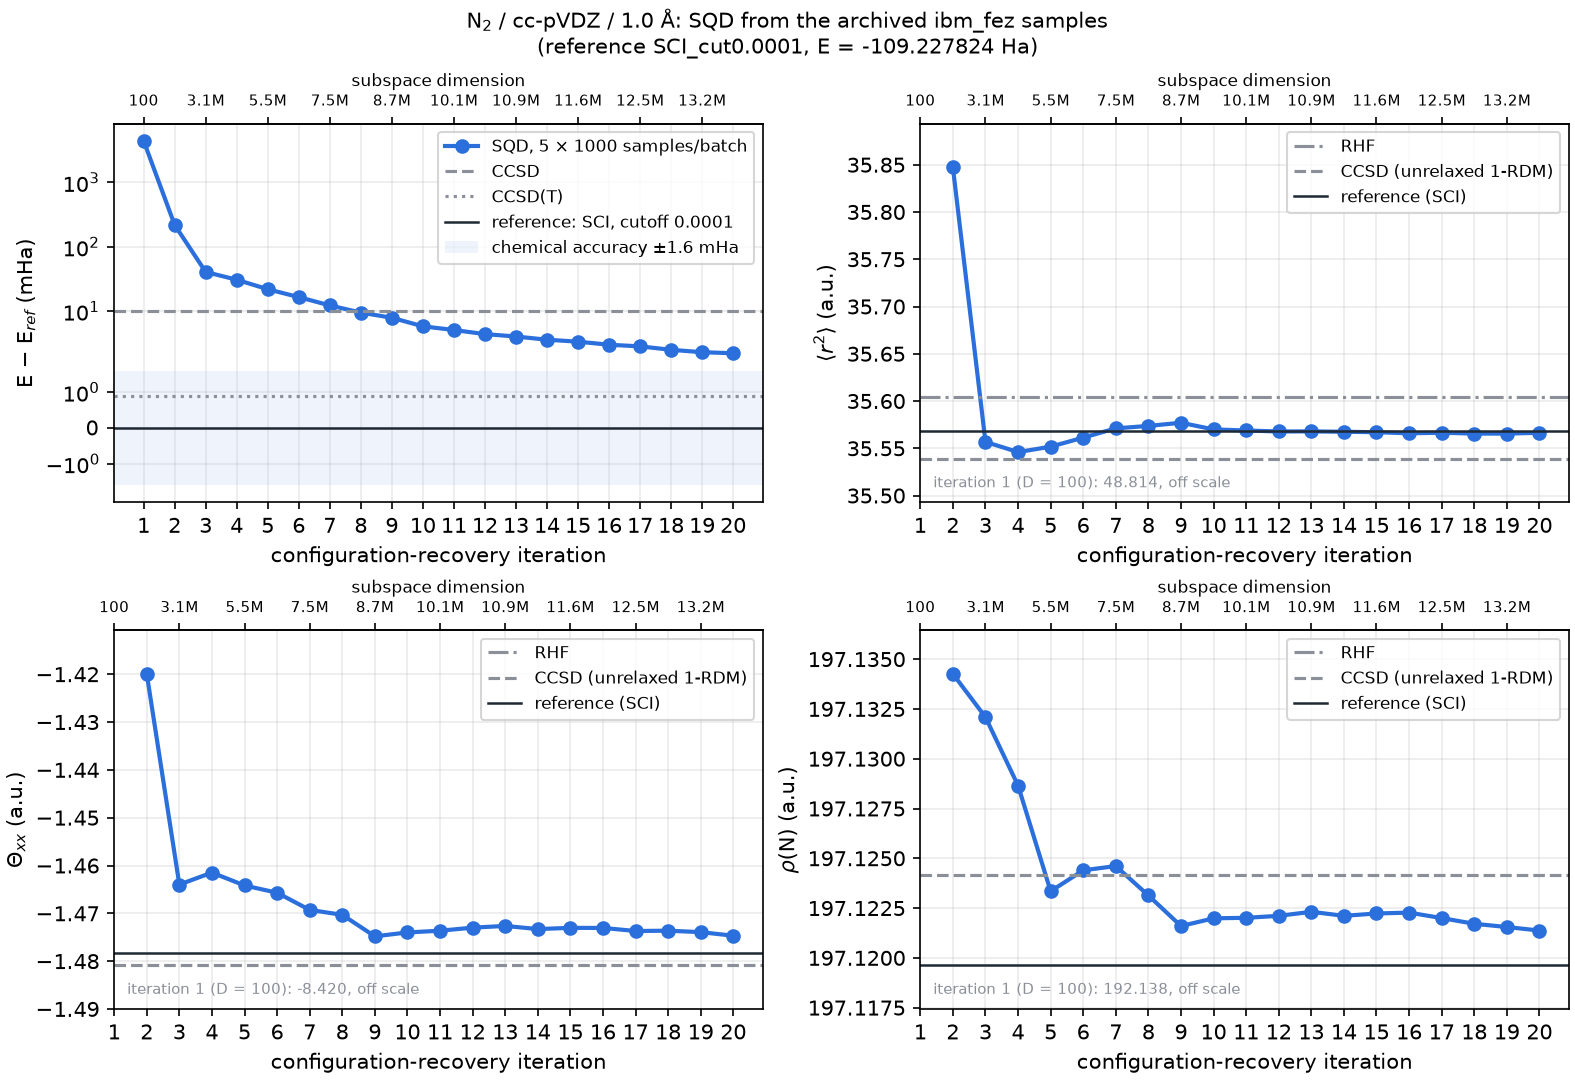
\includegraphics[width=\linewidth]{figures/property_curve_prod.png}
\caption{N$_2$ / cc-pVDZ / 1.0 \AA{}, SQD from the archived ibm\_fez samples: energy error (symlog scale, with CCSD, CCSD(T), the selected-CI reference and the $\pm$1.6 mHa band) and the three one-body properties as functions of the configuration-recovery iteration, subspace dimension on the upper axis; RHF, CCSD and the reference as horizontal lines. Iteration 1 (100 determinants) is off every property axis and annotated.}\label{fig:1}
\end{figure}


\subsection{The fork}\label{sec:3.3}


\begin{figure}[htbp]
\centering
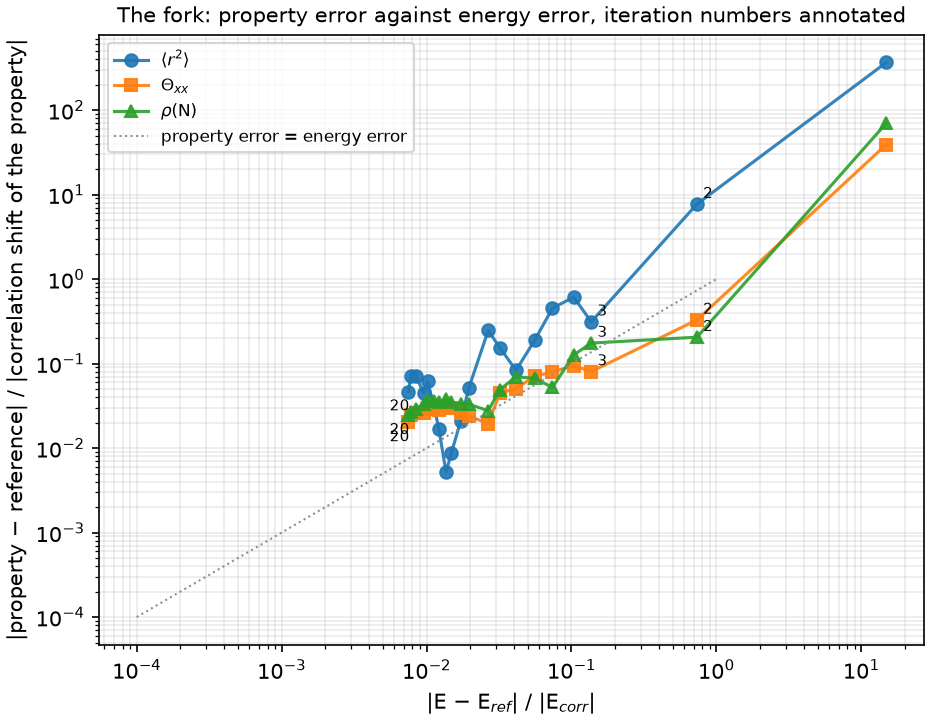
\includegraphics[width=\linewidth]{figures/fork_prod.png}
\caption{The fork: error of each property, in units of its correlation shift, against the energy error in units of the correlation energy, both relative to the selected-CI reference, log--log, with the iteration numbers annotated and the diagonal on which the two errors would be equal.}\label{fig:2}
\end{figure}


Figure 2 places the three properties on the pre-print's diagnostic plot \cite{ECGseedingSQD}. From iteration 5 to 9 the quadrupole and the contact density run along the diagonal; from iteration 9 to 20 they move horizontally, the energy axis advancing while the property axis does not, and end a factor of three above the diagonal. The second moment scatters above the diagonal by up to an order of magnitude through iteration 9, dives through it at iteration 12, and climbs back to a factor of six above it by iteration 20; nothing on the energy axis marks either turn. The plot also shows where CCSD would sit: 3.4 \% on the energy axis, and 80 \%, 1.5 \% and 6.3 \% on the three property axes --- the same ordering, the same outlier.

\textbf{Summary.} The fork between energy and property fidelity exists on N$_2$, but it is narrow and it is selective: it opens for the observable that weights the density where the subspace is thinnest.

\subsection{What the samples contain}\label{sec:3.4}


The archived 50 000 bitstrings have a mean Hamming weight of 23.97 of 52 for a state with 10 electrons; five of them, 0.01 \%, lie in the ($5\alpha$, $5\beta$) sector, all 50 000 are distinct, and every qubit is occupied between 39 \% and 53 \% of the time. The first diagonalization of the run of record is built on those five shots and spans 100 determinants at $-$104.80 Ha; every later subspace, 2.7 million determinants and $-$109.01 Ha at iteration 2 through 13.7 million and $-$109.2255 Ha at iteration 20, is produced by configuration recovery flipping the bits of the remaining samples toward the occupations of the current eigenvector, followed by diagonalization. The energies and properties of this paper are therefore those of a classical selected-configuration method with an occupancy-biased configuration generator whose seeds are five valid hardware shots and whose raw material is the remaining 49 995 strings, repaired. That uniform noise can stand in for the samples once the subspace is allowed to grow has been reported independently \cite{vanRossum2026}; the controls of this paper ask the same question with the schedule of the run of record fixed and the properties graded. Two of them are the control the published work does not contain, a subspace seeded by a classical coupled-cluster prior compared with the hardware seed at matched size; the only ablation in the published work is against uniformly random in-sector strings \cite{SQD,IBMdata}. Four controls have reported (Table 4, Figure 3). In the first, the 50 000 hardware bitstrings are replaced by uniformly random 52-bit strings, five of them drawn uniformly from the ($5\alpha$, $5\beta$) sector so that the loop starts from the same number of valid seeds as the hardware set; uniform noise alone contains none, the expected count being 0.05, and the loop cannot start without one. In the second, the hardware samples are kept and the first recovery iteration is primed with the CCSD natural occupations of the active orbitals instead of the occupations of the five valid shots. In the third, the hardware samples are kept and the 5 000 largest determinants of the CCSD wavefunction, 778 $\alpha$ and 778 $\beta$ strings, are forced into every subspace. In the fourth, all 50 000 strings are drawn uniformly from the right particle sector, the control design of the run of record \cite{SQD}.


\begin{table}[htbp]
\centering
\caption{Energy in hartree and subspace dimension by recovery iteration: the hardware samples, random strings with five random valid seeds, hardware samples with a CCSD-occupation prior, and hardware samples with the CCSD configurations forced in; the in-sector control, whose loop is static, is given in the text and in Table 5. The hardware run is continued to iteration 9 so that the priors' last points can be read against it at equal subspace size.}\label{tab:4}
\small
\renewcommand{\arraystretch}{1.3}
\begin{tabularx}{\linewidth}{@{}ll>{\hsize=0.901\hsize\raggedright\arraybackslash}Xl>{\hsize=1.099\hsize\raggedright\arraybackslash}X@{}}
\toprule
iteration & hardware samples & random strings, five valid seeds & CCSD-occupation prior & hardware, CCSD configurations forced in \\
\midrule
1 & $-$104.8012 (100) & $-$91.9885 (100) & $-$109.1750 (2.49 M) & $-$109.2151 (0.62 M) \\
2 & $-$109.0092 (2.75 M) & $-$105.6962 (2.60 M) & $-$109.1918 (3.88 M) & $-$109.2170 (4.45 M) \\
3 & $-$109.1870 (3.12 M) & $-$108.9603 (2.81 M) & $-$109.2024 (4.76 M) & $-$109.2187 (5.70 M) \\
4 & $-$109.1969 (4.36 M) & $-$109.1735 (3.23 M) & $-$109.2082 (5.94 M) & $-$109.2203 (6.71 M) \\
5 & $-$109.2058 (5.52 M) & $-$109.1978 (4.17 M) & $-$109.2133 (6.83 M) & $-$109.2213 (7.77 M) \\
6 & $-$109.2112 (6.66 M) & $-$109.2060 (5.44 M) & $-$109.2171 (7.77 M) & $-$109.2222 (8.51 M) \\
7 & $-$109.2155 (7.47 M) &  &  &  \\
8 & $-$109.2183 (8.08 M) &  &  &  \\
9 & $-$109.2199 (8.71 M) &  &  &  \\
\bottomrule
\end{tabularx}
\end{table}



\begin{table}[htbp]
\centering
\caption{The three properties at iteration 6 (iteration 3 for the in-sector strings, whose loop is static), deviation from the selected-CI reference as a percentage of the correlation shift.}\label{tab:5}
\small
\renewcommand{\arraystretch}{1.3}
\begin{tabularx}{\linewidth}{@{}>{\hsize=1.000\hsize\raggedright\arraybackslash}Xllll@{}}
\toprule
samples & $\Delta E$ (mHa) & \begin{tabular}[b]{@{}l@{}}$\langle r^{2}\rangle$\\error (\%)\end{tabular} & \begin{tabular}[b]{@{}l@{}}$\Theta_{xx}$\\error (\%)\end{tabular} & \begin{tabular}[b]{@{}l@{}}$\rho(\mathrm{N})$\\error (\%)\end{tabular} \\
\midrule
hardware samples & 16.6 & 19 & 7.1 & 6.7 \\
random strings, 5 random seeds & 21.8 & 24 & 14.9 & 14.3 \\
CCSD-occupation prior & 10.7 & 13 & 1.0 & 3.0 \\
CCSD-configuration prior & 5.6 & 3 & 2.6 & 6.8 \\
uniform in-sector strings & 2098 & 12 000 & 330 & 1 300 \\
\bottomrule
\end{tabularx}
\end{table}


\begin{figure}[htbp]
\centering
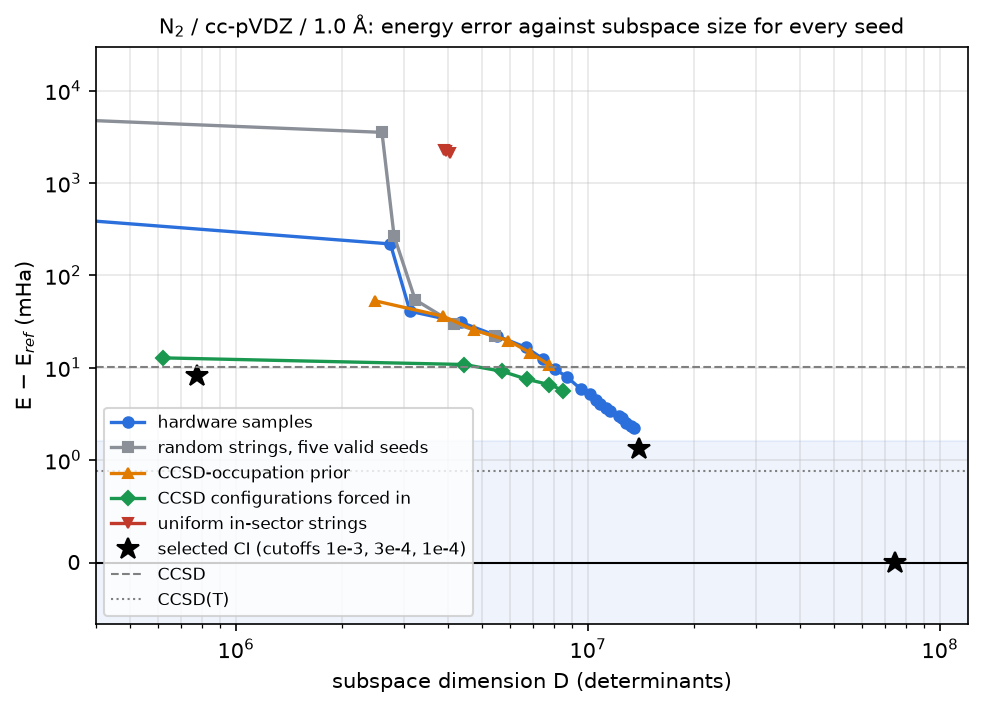
\includegraphics[width=\linewidth]{figures/controls_equal_D.png}
\caption{Energy error against subspace dimension for the hardware run and the four controls, with the three selected-CI points; symlog error scale, $\pm$1.6 mHa band, CCSD and CCSD(T) as horizontal lines; every point of the five seeds is on the scale, the in-sector control two hartree above the rest. Equal-size comparisons read vertically.}\label{fig:3}
\end{figure}


Random strings with five random valid seeds start 12.8 Ha above the hardware seed and follow the hardware run with a lag of one recovery iteration: at iteration 6 they match the hardware run at iteration 5 to 0.2 mHa, on a subspace a fifth smaller. The CCSD-occupation prior skips the seed stage, its first subspace is already the size of the hardware run's second, and it keeps the loop one and a half to two iterations ahead at equal iteration. At equal subspace size the advantage vanishes: its 7.8-million-determinant point lies between the hardware run's 7.5- and 8.1-million points. The prior buys growth of the subspace, not a better subspace. The properties say the same with one addition. With the prior the quadrupole and the contact density reach 1 \% and 3 \% of their shifts at iteration 6, where the hardware run stands at 7 \%, while the second moment swings between $-$1 \% and $-$28 \% across the six iterations exactly as it does in the hardware run: occupations carry no information on the single-excitation content of the state, which the second moment reads and the energy does not. The CCSD-configuration prior supplies exactly that content. Its first subspace, 0.62 million determinants, already has the energy the hardware run reaches at iteration 7 with 7.5 million; at equal size, 8.5 against 8.7 million, it is 2.3 mHa below the hardware run, the only control that beats it at matched subspace size; and its second moment never swings, staying between 1 \% and 5 \% of its shift on the low side through all six iterations. The prior fixes the observable it carries information about and no other: the contact density starts at 18 \% with this prior and converges slowly to 7 \%, because the largest CCSD determinants carry the valence tail and not the core-region doubles the contact density needs. The fourth control confirms what the loop is made of. When every string is valid, the recovery has nothing to repair and each iteration only re-subsamples the same 50 000 random configurations: three iterations at 3.9 to 4.0 million determinants give $-$106.95, $-$107.04 and $-$107.13 Ha, 1.8 Ha above Hartree--Fock and 2.1 Ha above the reference, with the second moment 4 to 6 a.u. off. This is the control design of the run of record, and on N$_2$ it says what it said on the iron--sulfur clusters: hardware samples beat in-sector noise by a wide margin. The comparison that carries information is the other one. The raw material of the loop is the invalid strings, repaired toward the occupations of the current eigenvector: uniform noise supplies that material one iteration late and, at equal subspace size, as well as the device does, and a classical prior supplies the occupations it is repaired toward as well as the device does, or better.

\textbf{Summary.} At 3 790 two-qubit gates on a Heron processor the sampled state carries no measurable particle-number structure, and what the device contributed to the published energy is a seed. The published work's own control is confirmed: hardware samples beat uniform in-sector strings by two hartree here and by 2.6 hartree on the iron--sulfur cluster, a margin the loop cannot close. The controls the published work did not run give the rest of the picture: at equal iteration the seed is worth one recovery iteration over random seeds; at equal subspace size it is worth nothing against random seeds or a classical occupation prior, and less than a classical configuration prior (Table 11).

\subsection{Where the prior fails}\label{sec:3.5}


The recovery loop repairs strings toward a product of orbital occupations, and where the strings carry no structure of their own it generates configurations from that product. It fails where the exact configuration weights are far from any product of marginals, and that distance can be measured before a molecule is chosen. For each system in Table 6 an exact or selected-CI reference in the stated active space gives the weights w and, from its one-particle density, the product prior q the loop repairs toward. $\mathrm{KL}(w\,\|\,q)$ is the information no occupancy-driven generator can see, a bound on what the loop's proposals carry; the Hartree--Fock weight and the NOON count locate the failure, and the CCSD diagnostics are given for comparison (definitions in Table 1).


\begin{table}[htbp]
\centering
\caption{The product prior against the exact weights, sorted by the Hartree--Fock weight. Active spaces in cc-pVDZ with frozen cores unless stated (H$_6$ and H$_8$ in STO-3G; the 8-site Hubbard ring at half filling in the site basis); N$_2$, C$_2$ and F$_2$ at selected-CI cutoff $10^{-3}$, the rest exact. $\rho$ is the Spearman rank correlation; * = zero by symmetry.}\label{tab:6}
\footnotesize
\renewcommand{\arraystretch}{1.15}
\begin{tabular}{@{}llllllll@{}}
\toprule
system & space & KL (bits) & KL/pair & $\rho$ & $w_{\mathrm{HF}}$ & NOONs & T1 \\
\midrule
BeH$_2$, x = 2.75 bohr & (4e,23o) & 1.35 & 0.68 & 0.27 & 0.00 & 4 & 0.044 \\
C$_2$ at 1.2425 \AA{} & (8e,26o) & 2.07 & 0.52 & 0.31 & 0.00 & 7 & 0.038 \\
Hubbard, U/t = 8 & (8e,8o) & 5.67 & 1.42 & 0.00 & 0* & 8 & --- \\
Hubbard, U/t = 4 & (8e,8o) & 3.81 & 0.95 & 0.01 & 0* & 8 & --- \\
N$_2$ at 2.5 \AA{} & (10e,26o) & 4.28 & 0.86 & 0.41 & 0.12 & 8 & 0.037 \\
H$_8$ chain 2.0 \AA{} & (8e,8o) & 3.40 & 0.85 & 0.11 & 0.21 & 8 & 0.074 \\
H$_6$ ring 2.0 \AA{} & (6e,6o) & 2.97 & 0.99 & 0.11 & 0.30 & 6 & 0* \\
N$_2$ at 2.0 \AA{} & (10e,26o) & 3.52 & 0.70 & 0.47 & 0.34 & 8 & 0.038 \\
Be$_2$ at 2.45 \AA{} & (4e,26o) & 1.72 & 0.86 & 0.33 & 0.79 & 7 & 0.027 \\
O$_3$ (C2v) & (12e,12o) & 1.49 & 0.25 & 0.69 & 0.81 & 7 & 0.034 \\
F$_2$ at 1.41 \AA{} & (14e,26o) & 1.27 & 0.18 & 0.36 & 0.89 & 4 & 0.010 \\
N$_2$ 1.0 \AA{} (this work) & (10e,26o) & 1.13 & 0.23 & 0.51 & 0.90 & 6 & 0.009 \\
BeH$_2$, linear & (4e,23o) & 0.65 & 0.32 & 0.27 & 0.96 & 3 & 0.006 \\
\bottomrule
\end{tabular}
\end{table}


Along the N$_2$ dissociation the prior loses three to four times its information while the ordering of the configurations survives, the rank correlation staying near one half: the loop would still find the right determinants and misjudge their weights. Configuration switches, BeH$_2$ at its transition and C$_2$ at equilibrium, remove the aufbau determinant from the state altogether. The Hubbard ring at half filling has a uniform prior by symmetry, so its divergence is the entropy the sampler would have to supply, and it grows monotonically with U/t. F$_2$, ozone, Be$_2$ and N$_2$ at equilibrium are where the loop is comfortable, which is where every published demonstration sits.

The largest system of the published work is a case in point. For the [4Fe-4S] cluster in its (54e, 36o) active space, the data archive of the run of record \cite{IBMdata}, which is not referenced from the paper's data statement, provides the integrals in the canonical basis of the hardware samples, the 3.16 million shots, the energies of the SQD batches at subspace sizes from 4 to 100 million determinants, an in-sector uniform control, and the classical references. CCSD in that basis has a T1 diagnostic of 0.099 and leaves twenty natural occupations fractional, so the recovery loop's prior fails there by every diagnostic of Table 6 that can be evaluated without an exact reference. The archive's own numbers then read as follows. The hardware run's best batch at 100 million determinants, $-$326.645 Ha, lies 0.19 Ha above CCSD, 0.15 Ha above the best heat-bath CI and 0.59 Ha above DMRG, and 1.8 Ha below the in-sector uniform control at 4 million. Of the 3.16 million shots, 1 694, or 0.054 \%, lie in the right particle sector, and all shots are distinct (Table 7). Where the prior fails most, the sampler is graded against the weakest control, and the energy is the only thing graded.


\begin{table}[htbp]
\centering
\caption{The [4Fe-4S] numbers of the data archive \cite{IBMdata}; the archive directories are experiments/4Fe-4S (samples, energetics, uniform control), classical\_reference\_energies/4Fe-4S and integrals/4Fe-4S.}\label{tab:7}
\small
\renewcommand{\arraystretch}{1.3}
\begin{tabularx}{\linewidth}{@{}>{\hsize=1.031\hsize\raggedright\arraybackslash}X>{\hsize=0.779\hsize\raggedright\arraybackslash}X>{\hsize=1.191\hsize\raggedright\arraybackslash}X@{}}
\toprule
quantity & value & where in the archive \\
\midrule
shots, all distinct & 3 163 742 & the measurement-outcomes pickle (April 2024 job IDs) \\
shots in the (27, 27) sector & 1 694 (0.054 \%) & same \\
mean Hamming weight, 72 bits for 54 electrons & 42.2 & same \\
best SQD batch of 100 at d = 100 M & $-$326.6448 Ha & hardware energetics, d = 100 M file \\
best SQD batch of 100 at d = 9 M & $-$326.5918 Ha & hardware energetics, d = 9 M file \\
SQD energy--variance point at d = 4 M & $-$326.5560 Ha & hardware energy--variance file \\
in-sector uniform control at d = 4 M & $-$324.7678 Ha & uniform-distribution energy--variance file \\
RHF, CISD, CCSD & $-$326.5474, $-$326.7421, $-$326.8376 Ha & classical reference energies file \\
HCI (best), DMRG & $-$326.7939, $-$327.2396 Ha & same \\
CCSD in the sample basis, this work & T1 0.099; 20 fractional NOONs & computed from the FCIDUMP \\
\bottomrule
\end{tabularx}
\end{table}


The ranking selects N$_2$ at 2.0 to 2.5 \AA{} in a (10e, 16o) window as the case to measure: it keeps this paper's molecule and properties, breaks the CCSD prior, and its 19-million-determinant sector admits both an exact reference and exact sampling of the circuit state, so that the information carried by the seed is the only variable.

\textbf{Summary.} The failure of the recovery loop's prior is measurable in advance, and it is not where SQD has been demonstrated.

\subsection{The measurement where the prior fails}\label{sec:3.6}


\subsubsection{\texorpdfstring{Nitrogen molecule (N$_2$)}{Nitrogen molecule (N2)}}\label{sec:3.6.1}


N$_2$ is taken to twice and two and a half times its equilibrium distance in a (10e, 16o) window of the 6-31G basis, the active space of the published 6-31G run and of DF-SQD \cite{AgarwalRay2026}, on the bond lengths of the data archive \cite{IBMdata}. In that space the sector holds 19.1 million determinants, so the reference is full CI, computed here and agreeing with the archive's table to a microhartree, and the LUCJ state built from the CCSD amplitudes can be sampled exactly.

Six seeds run the loop of \S\ref{sec:2.4} for ten iterations at every geometry: 50 000 exact samples of the LUCJ state; the archive's 100 000 hardware shots at the same geometry, relabelled to the present orbital order after a check that the two integral sets coincide to $10^{-4}$ and that a batch diagonalized in either basis gives the same energy to $4\times10^{-6}$ Ha; uniform noise with five random valid strings; the hardware shots with the CCSD-occupation prior; the hardware shots with the CCSD configurations forced in; and uniformly random in-sector strings.


\begin{table}[htbp]
\centering
\caption{Energies in hartree after ten recovery iterations (two for the exact LUCJ samples, whose loop is static; the exact evolved-state samples converge within their support in nine iterations at equilibrium and run the full ten at 2.744 \AA{}, still descending), against full CI; the coupled-cluster references, the number of distinct configurations among the 50 000 exact LUCJ samples and the full-CI weight those configurations carry are given for each geometry. At 2.744 \AA{} the coupled-cluster equations do not converge; the CCSD row, the LUCJ state and the two priors at that geometry are built from the unconverged amplitudes, which a rerun of the same script does not reproduce, the iteration stopping at a different amplitude set (55 distinct configurations in the rerun), so no weight is quoted there.}\label{tab:8}
\small
\renewcommand{\arraystretch}{1.3}
\begin{tabularx}{\linewidth}{@{}>{\hsize=1.000\hsize\raggedright\arraybackslash}Xlll@{}}
\toprule
 & R = 1.0975 \AA{} & R = 2.195 \AA{} & R = 2.744 \AA{} \\
\midrule
Hartree--Fock & $-$108.8678 & $-$108.2186 & $-$108.0384 \\
CCSD & $-$109.0935 & $-$108.9194 & $-$108.4658 \\
full CI, 19.1 M determinants & $-$109.1029 & $-$108.8477 & $-$108.8398 \\
exact LUCJ samples (distinct configurations; full-CI weight) & $-$109.0527 (142; 0.962) & $-$108.7510 (384; 0.730) & $-$108.7092 (293; ---) \\
exact evolved-state samples, t = 4 (distinct configurations) & $-$109.1008 (2146) & not run & $-$108.8310 (4764) \\
evolved samples through the bit-flip channel & $-$109.1017 & not run & $-$108.8356 \\
hardware shots & $-$109.1027 & $-$108.8471 & $-$108.8389 \\
random strings, five valid seeds & $-$109.1027 & $-$108.8470 & $-$108.8383 \\
CCSD-occupation prior & $-$109.1027 & $-$108.8472 & $-$108.8390 \\
CCSD configurations forced in & $-$109.1027 & $-$108.8472 & $-$108.8392 \\
uniform in-sector strings & $-$109.1027 & $-$108.8467 & $-$108.8389 \\
\bottomrule
\end{tabularx}
\end{table}


The exact samples of the circuit are the surprise of the table. Fifty thousand draws from the LUCJ state contain 142 distinct configurations at equilibrium, 384 at twice the distance and 293 at two and a half times, the first two sets carrying 0.962 and 0.730 of the full-CI weight; every one of them is valid, so the recovery has nothing to repair, the loop stops after two iterations, and the energy stays 50, 97 and 131 mHa above full CI, 41 mHa above CCSD at equilibrium. That is the coupon-collector limit measured directly: the state the circuit prepares is too concentrated for sampling to reach its tail, and the noisy device beats its own clean circuit because the invalid strings that noise produces are the raw material of the recovery. With that material present, the seeds converge to the same place. At equilibrium the hardware shots, uniform noise with five seeds, the occupation prior and even uniform in-sector strings all end within 0.2 mHa of full CI, because in a space of 4 368 strings per spin, 50 000 uniform in-sector draws almost surely contain every string, the expected number missed being 0.05, and carry-over does the rest. At twice the distance, where CCSD overshoots full CI by 72 mHa and the prior fails by the diagnostics of Table 6, the five active seeds end within 0.5 mHa of one another, the two coupled-cluster priors ahead of the hardware shots by 0.1 to 0.2 mHa, the hardware shots ahead of noise by 0.1 mHa, and in-sector strings, which this small space lets the loop improve, 0.3 mHa behind the hardware shots. At two and a half times the distance the coupled-cluster equations no longer converge and the CCSD energy stops 374 mHa above full CI, yet the occupations and the leading configurations of that unconverged solution remain the best seeds. After ten iterations the configuration prior is 0.65 mHa above full CI, the occupation prior 0.76, the hardware shots 0.91, noise with five seeds 1.54, and in-sector strings 0.89 in a subspace 1.6 times larger than the hardware one. At equal subspace size the ordering is sharper: near 4.9 million determinants the configuration prior is 0.8 mHa above full CI, the occupation prior and the hardware shots 0.9, noise with five seeds 1.5 at 4.5 million, and in-sector strings 49. Along the iterations the picture of \S\ref{sec:3.4} repeats at every geometry: at the third and the fifth iteration the occupation prior carries about half the error of the hardware shots, and the hardware shots about half the error of noise, a one-iteration head start over noise and a one-iteration lag behind the prior. The head start is not a shot-count artefact: the hardware seed used the archive's 100 000 shots against 50 000 strings for the random and in-sector seeds, and a repeat with 50 000 of the archive's shots costs the hardware seed 0 to 7 mHa at the third iteration and nothing at the tenth, leaving it ahead of the random seed at the third iteration by 2 to 11 mHa at the three geometries and level with it at the end. The properties do not discriminate at all. Every seed that reaches the millihartree reproduces the full-CI $\langle r^{2}\rangle$ to 0.01 a.u. and the quadrupole to 0.01 a.u. at every geometry, with $\langle S^{2}\rangle$ below $10^{-3}$. So the failure of the prior in energy does not reach its first moment: the occupations of a coupled-cluster solution whose energy is 374 mHa wrong are still, to the precision the recovery step consumes, the right occupations. The diagnostics of Table 6 select the geometries where the prior's energy fails; they do not predict that its seed will, and here it does not.

\subsubsection{Iron--sulfur cluster ([4Fe-4S])}\label{sec:3.6.2}


The [4Fe-4S] run of Table 7 is the case the diagnostics rank hardest for a product prior, twenty fractional natural-orbital occupations and a $T_{1}$ of 0.10, and its archive holds everything the controls need except a solver: at 36 orbitals the selected-CI solver of \S\ref{sec:2.4} takes 26 s per matrix--vector product. The four seeds were therefore run through the same loop with the sbd eigensolver of RIKEN \cite{sbd} on eight MPI ranks, two batches of 1 000 samples and three recovery iterations, with $\langle S^{2}\rangle$ computed from the saved eigenvector and no spin penalty, as in the \S\ref{sec:3.4} rerun and unlike the stretched-N$_2$ seeds of \S\ref{sec:3.6}.1. Table 9 gives the result. The hardware shots reach $-$326.577 Ha at 4.26 M determinants, 21 mHa below the archive's own value at that size, so the loop lands on the published energy at that size. The CCSD-occupation prior reaches that energy one iteration earlier and ends 12 mHa lower at a subspace 12 \% larger; at equal subspace size, its second iteration against the hardware's third, the two agree within 3 mHa. The configurations of a coupled-cluster solution that itself does not converge, 833 strings per spin from its top 5 000 determinants, sit 155 mHa lower still at twice the subspace, 1 mHa below CISD, and a repeat with 600 samples per batch gives the same energies at 4.0 to 4.3 million determinants, $-$326.743 Ha, 1 mHa below CISD and 166 mHa below the hardware shots at equal subspace size. That state is not a pure singlet: its $\langle S^{2}\rangle$ is 0.068 at either size and every iteration, against 0.006 for the hardware seed and 0.050 for the occupation prior at the end of their loops, so the forced configuration set, spin-symmetric as a set of strings but not spin-complete, leaves a little of the cluster's nearby higher-spin character in the lowest state. The spin penalty of \S\ref{sec:3.7} settles what that costs: with $\lambda$ = 0.2 the configuration prior's state has $\langle S^{2}\rangle$ = 0.014, its energy rises by 3 mHa, and it remains 163 mHa below the hardware seed at equal subspace size and 2 mHa above CISD at 8 million. The lead is a singlet lead. With 2 000 samples per batch the hardware shots reach $-$326.603 Ha at 17.12 M determinants, the archive's own value at 16 million, so the loop lands on the published energies at both sizes. Uniform in-sector strings are static at 2.6 Ha above Hartree--Fock, as the exact circuit samples were in Table 8, because nothing invalid remains to repair and 2 000 random strings out of the $9\times10^{15}$ determinants of the sector do not couple. The reading of \S\ref{sec:3.4} therefore repeats on the largest published run: a one-iteration head start over noise, none over the occupation prior at equal subspace size, and a configuration prior whose lead survives the spin penalty. Two cautions belong with it. Without a spin penalty $\langle S^{2}\rangle$ drifts upward as the subspace grows, from 0.009 to 0.050 for the occupation prior and to 0.07 for the hardware shots at 17 million determinants, and one raw hardware batch, before any recovery, converged onto a state with $\langle S^{2}\rangle$ = 0.74; the published run reports no $\langle S^{2}\rangle$. And the schedule here is a fraction of the published one. The archive's energetics files hold one hundred batches at each of five subspace sizes from 9 to 100 million determinants, the published run reports its best batch at each size after its full configuration-recovery schedule, and its eigensolver carried a penalty of the squared form, $\lambda$($S^{2}$ $-$ s(s+1))$^{2}$, where the penalty used here is linear in $S^{2}$. Three iterations on two batches of 1 000 samples are therefore equal-schedule comparisons between seeds at 4 to 17 million determinants, not reproductions of the published energies, which the loop nevertheless meets at the two sizes where they overlap.


\begin{table}[htbp]
\centering
\caption{The four seeds of \S\ref{sec:3.4} on the archived [4Fe-4S] run \cite{IBMdata} ((54e, 36o), 3.16 million hardware shots of which 1 694 are in the sector): energy in hartree after each of three recovery iterations with two batches of 1 000 samples, the sbd eigensolver, no spin penalty unless stated; final subspace dimension and $\langle S^{2}\rangle$ of the final state, computed from the saved eigenvector in the alpha-first convention (\S\ref{sec:3.7}). Rows five and six are the equal-size pair: the configuration prior at the hardware seed's subspace size, and the hardware seed at the archive's 16 M size. The last two rows repeat the configuration prior with the spin penalty of \S\ref{sec:3.7}, $\lambda$ = 0.2; their energies are $\langle$H$\rangle$ of the eigenvector of H + $\lambda$$S^{2}$. Archive references: RHF $-$326.547, CISD $-$326.742, CCSD $-$326.838, HCI $-$326.794, DMRG $-$327.240; the archive's own hardware batches $-$326.556 at 4 M, $-$326.592 at 9 M and $-$326.603 at 16 M determinants, its uniform in-sector control $-$324.768 at 4 M.}\label{tab:9}
\footnotesize
\renewcommand{\arraystretch}{1.15}
\begin{tabularx}{\linewidth}{@{}>{\hsize=1.000\hsize\raggedright\arraybackslash}Xlllll@{}}
\toprule
seed & iteration 1 & iteration 2 & iteration 3 & final D & final $\langle S^{2}\rangle$ \\
\midrule
hardware shots & $-$326.079 & $-$326.447 & $-$326.577 & 4.26 M & 0.006 \\
CCSD-occupation prior & $-$326.553 & $-$326.579 & $-$326.589 & 4.77 M & 0.050 \\
CCSD configurations forced in & $-$326.742 & $-$326.743 & $-$326.743 & 8.59 M & 0.068 \\
uniform in-sector strings & $-$323.957 & $-$323.957 & $-$323.957 & 4.01 M & 0.000 \\
CCSD configurations forced in, 600 samples per batch & $-$326.742 & $-$326.742 & $-$326.743 & 4.31 M & 0.067 \\
hardware shots, 2 000 samples per batch & $-$326.080 & $-$326.578 & $-$326.603 & 17.12 M & 0.066 \\
CCSD configurations, 600 samples per batch, spin penalty & $-$326.739 & $-$326.739 & $-$326.739 & 4.24 M & 0.014 \\
CCSD configurations, spin penalty & $-$326.739 & $-$326.740 & $-$326.740 & 8.40 M & 0.015 \\
\bottomrule
\end{tabularx}
\end{table}


\subsubsection{A broader sampler, measured}\label{sec:3.6.3}


The clean-circuit result asks for a state whose exact samples are numerous and broad, and the published candidate is the time-evolved Hartree--Fock state \cite{MikkelsenNakagawa2025}. It can be measured exactly in a window small enough for everything to cost seconds: the lowest twelve active orbitals of the 6-31G space at equilibrium, (10e, 12o), a sector of 627,264 determinants whose full CI takes nine seconds. Fifty thousand exact shots are drawn from the one-layer LUCJ state built from the CCSD amplitudes of that window and from exp($-$iHt)|HF$\rangle$, evolved exactly by a Krylov exponential for a scan of t; for each sample set Table 10 gives the number of distinct configurations, the number of distinct $\alpha$ strings, the full-CI weight the sampled determinants carry, and the energy of the loop of \S\ref{sec:2.4} on those samples, which is static because every sample is valid.


\begin{table}[htbp]
\centering
\caption{Exact samples of the one-layer LUCJ circuit and of the time-evolved state in the (10e, 12o) window of N$_2$ at 1.0975 \AA{}, 50 000 shots each, and the static loop on them, given as its energy above full CI; full CI $-$108.999490 Ha, Hartree--Fock $-$108.867774 Ha. ``CCSD amplitudes'': parameters read from the coupled-cluster amplitudes; ``optimized to convergence'': parameters minimized against the exact energy of the window (linear method, $10^{-8}$ relative test), as ranges over the independent optimizations described in the text. 1 $-$ W(U$\times$U): the full-CI weight missing from the product space of the sample's $\alpha$ and $\beta$ strings, the space the static loop diagonalizes in. The two closing rows take full CI's own largest determinants as the sample.}\label{tab:10}
\footnotesize
\renewcommand{\arraystretch}{1.15}
\begin{tabularx}{\linewidth}{@{}>{\hsize=1.000\hsize\raggedright\arraybackslash}Xlllll@{}}
\toprule
state sampled & \begin{tabular}[b]{@{}l@{}}distinct\\configurations\end{tabular} & $\alpha$ strings & \begin{tabular}[b]{@{}l@{}}full-CI weight\\captured\end{tabular} & \begin{tabular}[b]{@{}l@{}}static\\loop (mHa)\end{tabular} & 1 $-$ W(U$\times$U) \\
\midrule
LUCJ, all-to-all, CCSD amplitudes & 37 & 16 & 0.977 & 30.63 & $1.8\times10^{-2}$ \\
LUCJ, hardware pattern, CCSD amplitudes & 18 & 10 & 0.958 & 43.14 & $2.4\times10^{-2}$ \\
LUCJ, hardware pattern, optimized to convergence & 233--269 & 68--70 & 0.987--0.989 & 6.0--7.6 & $2.4\times10^{-3}$ to $3.9\times10^{-3}$ \\
LUCJ, all-to-all, optimized to convergence & 177--256 & 47--74 & 0.988--0.997 & 2.3--16.4 & $8.0\times10^{-4}$ to $1.1\times10^{-2}$ \\
evolved HF, t = 0.25 & 143 & 53 & 0.994 & 5.10 & $1.9\times10^{-3}$ \\
evolved HF, t = 0.5 & 274 & 86 & 0.998 & 1.83 & $6.3\times10^{-4}$ \\
evolved HF, t = 1.0 & 547 & 157 & 0.999 & 0.78 & $2.3\times10^{-4}$ \\
evolved HF, t = 2.0 & 631 & 162 & 0.998 & 0.58 & $1.5\times10^{-4}$ \\
evolved HF, t = 4.0 & 756 & 213 & 0.998 & 0.43 & $1.1\times10^{-4}$ \\
evolved HF, t = 8.0 & 832 & 229 & 0.998 & 0.48 & $1.2\times10^{-4}$ \\
full CI, 204 largest determinants & 204 & 65 & 0.998 & 3.09 & $9.4\times10^{-4}$ \\
full CI, 756 largest determinants & 756 & 158 & 1.000 & 0.58 & $1.5\times10^{-4}$ \\
\bottomrule
\end{tabularx}
\end{table}


Time evolution broadens the support by an order of magnitude over the one-layer LUCJ state, from 37 distinct configurations to 547 at t = 1 and 756 at t = 4, captures more of the full-CI weight, 0.977 against 0.998, and the all-valid static loop that stalled 31 mHa short on the LUCJ samples reaches half a millihartree. The evolved state's own energy stays at the Hartree--Fock value throughout, so it is a broad sampler rather than a good energy state, which is exactly the point: what the loop needs from the sampler is coverage, and the energy of the sampled state says nothing about it. Two cautions belong here. The static loop's subspace grows with t, from 361 to 69,169 determinants, so the captured weight per shot is the fair figure, and the gain saturates beyond t $\approx$ 2. And this is a twelve-orbital window; the same measurement in the sixteen-orbital space of Table 8, where a Krylov step costs minutes rather than seconds, is the next step.

The circuit's parameters are a variable the demonstrations do not use, and Table 10 measures it; its hardware pattern keeps the alpha--alpha interactions between neighbouring orbitals and the alpha--beta ones on the same orbital, as the heavy-hex layout does. The circuits sampled on hardware take their parameters from the coupled-cluster amplitudes without optimization, and the configuration prior of \S\ref{sec:3.4} is not that input but coupled cluster's output, the largest determinants of its wavefunction; the 2.3 mHa of Table 11 is what a sampled one-layer circuit loses against the amplitudes that parametrized it. Optimizing the parameters is the missing rung between the 142 and the 2 146 configurations of Table 8. In the window, the hardware pattern read from the amplitudes holds 18 configurations and its static loop stops 43 mHa short; optimized to convergence against the exact energy it holds 233--269 configurations, captures 0.987--0.989 of the full-CI weight and stops 6.0--7.6 mHa short, at an energy 42.5--43.7 mHa above full CI over three independent optimizations from the same start. For the hardware pattern the converged optimum is therefore reproducible to chemical accuracy in energy and to within a millihartree in what the loop does with its samples. The all-to-all circuit goes from 37 configurations and 30.6 mHa to 177--256 configurations and 2.3--16.4 mHa, but its three optimizations from the same start land in three optima, 9.2, 15.1 and 17.9 mHa above full CI, so its row is a range and not a value. A fourth optimization, started from the coupled-cluster parameters displaced by Gaussian noise of a tenth of their root-mean-square, which moves the start state from 37 to 215 sampled configurations, converged back to the third optimum, 18.0 mHa above full CI with a state overlap of 0.9996 with the third run's, so the three optima are the set the optimizer reaches from this neighbourhood and not an open-ended one; a fifteen-iteration snapshot of either circuit was not reproducible between runs. Optimization broadens a one-layer circuit's support by an order of magnitude and leaves it a factor of three to four below the evolved state's 756 configurations, with a static-loop error 5 to 38 times the evolved state's. The ordering of Table 10 is therefore one of circuit families, not of parameters: what the loop needs is support --- the strings whose product it diagonalizes in --- and a one-layer cluster-Jastrow circuit, however parametrized, concentrates its samples on a few hundred configurations.

The two circuits order differently by the state's energy and by the loop's, and both orderings have a reason. The all-to-all state lands closer to full CI in every run, by 25 to 34 mHa, its worst basin included. That is a containment, not a discrepancy: a one-layer circuit is an orbital rotation, a diagonal-Coulomb evolution and a second rotation, and setting the couplings the hardware pattern lacks to zero recovers it exactly, so the all-to-all manifold contains the hardware pattern's and its minimum cannot lie higher. The correlation the window holds is carried by double excitations between orbitals that are not neighbours in the ordering, which the restricted Jastrow cannot write directly; the 30 mHa between the two families is the price of the connectivity constraint, measured. The constraint is the processor's: the pattern is what a heavy-hex lattice executes without routing, and the reference tutorial, run on the square-lattice Nighthawk r2 processor ibm\_phoenix, switches the circuit's pass manager from heavy-hex to square connectivity \cite{Huang2026}, a pattern with more couplings per orbital that sits between the two rows of Table 10 and is a measurement for the next version; the same report puts a million samples in a minute on that processor, five times the rate of Heron r3 at similar result quality, which is the sampling budget a broader sampler would draw on. The larger manifold is also the rougher one: with 444 parameters against 311 and a local optimizer, the all-to-all circuit converges to three optima 9 mHa apart where the hardware pattern converges to one, and a perturbed start returns to one of the three. The loop's ordering is another matter, because the loop does not consume the state but its strings: it diagonalizes in the product of the $\alpha$ and $\beta$ strings the samples contain. Lowering the state's energy means getting the coefficients of the leading determinants right, which concentrates the samples. The two all-to-all optima at 15.1 and 17.9 mHa, the second reached twice, hold 177--186 configurations on 59--64 strings and their loops stop 12--16 mHa short, worse than the hardware pattern's 6 to 8 mHa on 88 to 93 strings; only the basin at 9.2 mHa, which spread over 256 configurations and 90 strings, hands the loop a better start at 2.3 mHa. A lower variational energy buys amplitude accuracy on the same few hundred configurations, not string diversity, and string diversity is what the loop pays for. The state's ordering is fixed by the family; the loop's is not fixed within this rung at all, which is the finding.

The quantity that does fix it is the last column of Table 10. The loop diagonalizes in the product space U $\times$ U of the $\alpha$ and $\beta$ strings a sample contains, and the full-CI weight that space misses, 1 $-$ W, orders every set in the table and every set of the exchange behind it: $1.1\times10^{-4}$ for the evolved state at t = 4 and 0.43 mHa; $1.5\times10^{-4}$ for full CI's own 756 largest determinants and 0.58; $8.0\times10^{-4}$ for the best all-to-all optimum and 2.3; $9.4\times10^{-4}$ for full CI's 204 largest determinants, whose 65 strings beat the hardware pattern's 88 to 93 strings at $2.4\times10^{-3}$ to $3.9\times10^{-3}$; $8.5\times10^{-3}$ to $1.1\times10^{-2}$ for the two narrow all-to-all optima and 12 to 16 mHa; $1.8\times10^{-2}$ and $2.4\times10^{-2}$ for the two circuits read from the amplitudes and 31 and 44. Neither the number of configurations nor the number of strings carries this ordering; the missing weight does, with one near-tie exchanged, the union of the two converged circuits at $1.2\times10^{-3}$ and 2.9 mHa against full CI's 204 at $9.4\times10^{-4}$ and 3.1. Two facts fix its meaning. The static loop's energy lies within 0.3 mHa of the energy of the normalized projection of the full-CI vector onto U $\times$ U for every converged set, and within 0.6 mHa for the two amplitude-read circuits, so the loop's diagonalization adds nothing the weight has not already decided. And the error divided by the missing weight runs from 1.4 to 4.1 Ha over the sets, an excitation-energy scale, so a static loop within a millihartree of full CI needs a string product that misses less than about $3\times10^{-4}$ of the weight: the evolved state has it from t = 1 on, and no one-layer circuit, whatever its parameters, does. The product space also misses three to four times less weight than the sampled configurations themselves, which is what the symmetric string product buys the loop, and why the loop is read here as consuming strings rather than configurations.

That step is now taken at equilibrium (Table 8, two added rows). In the sixteen-orbital space, 50 000 exact samples of the t = 4 state contain 2,146 distinct configurations against 142 for the LUCJ state, the first diagonalization on them stands 4.7 mHa above full CI against 50 mHa, and, because a batch of 1 000 holds only part of that support, the loop is no longer static: it keeps adding strings and converges within the sampled support at 2.1 mHa after 9 iterations. Passed through a bit-flip channel that leaves 6 \% of the strings valid, ten times the hardware's fraction, the same samples run the full loop and end at 1.2 mHa on 884 thousand determinants after ten iterations, where the hardware seed ends at 0.22 mHa on 3.4 million. At equal iteration the noisy evolved seed trails; at equal subspace size it leads, reaching at 533 thousand determinants the error the hardware seed reaches at 2.3 million. A broad sampler buys the loop accuracy per determinant; the hardware seed, with more to repair, buys it subspace growth.

At two and a half times the distance the repeat holds. The exact t = 4 samples hold 4 764 distinct configurations against 293 for the LUCJ state; the first diagonalization on them stands 32 mHa above full CI against 131, and ten iterations within the support bring the clean seed to 8.8 mHa on 1.0 million determinants, still descending, where the LUCJ samples are static. Through the channel, 6.4 \% valid, the noisy seed ends at 4.2 mHa on 1.7 million determinants after ten iterations, where the hardware shots end at 0.9 mHa on 4.9 million: at equal iteration it trails; at equal subspace size it leads, the hardware seed standing at 39 mHa on 1.8 million determinants and needing 3.6 million to reach 4 mHa, and the random seed at 34 mHa on 1.7 million. The reading of the equilibrium pair repeats where the prior fails: the evolved state buys accuracy per determinant, the hardware seed buys growth. The evolution itself cost three hours of the sixteen-orbital Krylov exponential at this geometry.

What no present device can do is prepare the evolved state itself: transpiled to the Heron gate set for the sixteen-orbital Hamiltonian, one first-order Trotter step of the double-factorized evolution costs 73 000 two-qubit gates with 33 factors and 150 000 with 81, before any routing, against 1 700 for the one-layer LUCJ circuit in the same sixteen-orbital space and 3 790 for the 52-qubit circuit of the run of record after routing to the heavy-hex lattice. At the published median two-qubit error of Heron r2, $2.5\times10^{-3}$, the sixteen-orbital LUCJ circuit survives with probability $10^{-2}$ and the circuit of the run of record with $10^{-4}$, the order of its 0.01 \% valid fraction, which the survival bounds from below since a string from a circuit that suffered an error can still be valid; at the $3.9\times10^{-3}$ of the fake-backend calibration snapshot the two figures are $10^{-3}$ and $4\times10^{-7}$, and a Trotter step survives with probability exp($-$180) to exp($-$280), while Nighthawk's announced budget is 5 000 two-qubit gates, 7 500 in 2026 and 10 000 in 2027 \cite{IBMNighthawk2025}. Two qualifications go with those numbers. The survival estimates are orders of magnitude, from a published median and from the calibration snapshot of the fake Heron r2 backend distributed with the runtime, ignoring readout, decoherence and mitigation, and the best Heron devices now report median two-qubit errors near $2\times10^{-3}$. And the count is specific to the dense double-factorized molecular Hamiltonian: sparse lattice and impurity Hamiltonians have been evolved on Heron processors at a few thousand two-qubit gates in the sample-based Krylov line \cite{Yu2025}, which is why that line runs on hardware first. The exact evolution is therefore a classical yardstick for what a broad sampler does; the route to a device is compression, and the 98 \% reduction against one Trotter step that generative circuit design reports at chemical precision on N$_2$ \cite{Kemmoku2026} would land at LUCJ scale, inside that budget.

\textbf{Summary.} Exact samples of the circuit cannot reach the tail; repaired noise can, from any source; and where the classical prior fails in energy, its occupations and its leading configurations still seed the loop at least as well as the hardware shots, whose contribution is a one-iteration head start over noise at equal iteration and a lead of 0.1 to 0.6 mHa at equal subspace size; and on the iron--sulfur cluster of the largest published run the same ordering holds, with the spin read alongside and a penalty confirming the classical seed's lead as a singlet energy.

\subsubsection{The classical solver's envelope, measured}\label{sec:3.6.4}


The reference implementation's documentation places its solver at about twenty-five spatial orbitals and ten electrons with subspace dimensions near 1$0^{7}$ on ten to thirty cores \cite{SQDaddonDocs}, and the run of record of \S\ref{sec:3.1}, (10e, 26o) at 13.5 million determinants, sits on that envelope. A sampler that covers the tail hands the solver larger subspaces than the circuit did, so the question of where the envelope ends, and how the cost grows toward it, is one this paper can answer on the machine that ran everything else. Table 12 measures it with the addon's own solver on the run of record's Hamiltonian. Two kinds of subspace are solved. The first are the subspaces the CCSD-configuration control recovered at each of its iterations, from 619 369 to 8 514 724 determinants; their energies were recorded when the control ran, and the solver here reproduces every one of the 17 recorded energies to within 2e-13 Ha, which validates the measurement against the paper's own results. The second are symmetric subspaces cut at random from the union of every string the controls saved, 19 884 $\alpha$ and 19 884 $\beta$ strings, 0.40 billion determinants in all, at dimensions from one to fifty million; their energies are not results, because a random cut of the pooled strings is not a subspace the loop would choose, and the table reports them only as timing points.


\begin{table}[htbp]
\centering
\caption{The classical solver of the loop on a sixteen-thread laptop (AMD Ryzen 7 6800H, 47 GB): qiskit-addon-sqd 0.12.1's \texttt{solve\_sci}, the selected-CI Davidson behind \texttt{solve\_fermion}, on the (10e, 26o) Hamiltonian of \S\ref{sec:3.1}, sixteen OpenMP threads, Davidson limit 200 cycles. The first block is the subspaces the CCSD-configuration control of \S\ref{sec:3.4} recovered at each iteration, where the recorded energy validates the solve; the second is symmetric subspaces cut at random from the union of every $\alpha$ and $\beta$ string the controls saved, up to the largest dimension the machine was asked to hold. Peak memory is the process's resident maximum after the solve.}\label{tab:12}
\footnotesize
\renewcommand{\arraystretch}{1.15}
\begin{tabular}{@{}lllllll@{}}
\toprule
subspace & \begin{tabular}[b]{@{}l@{}}strings\\per spin\end{tabular} & D & seconds & s per 1$0^{6}$ & peak GB & \begin{tabular}[b]{@{}l@{}}$\Delta$ vs recorded\\(Ha)\end{tabular} \\
\midrule
control, iteration 1 & 787 & 619 369 & 84 & 135 & 3.6 & +1e-13 \\
control, iteration 2 & 2 110 & 4 452 100 & 468 & 105 & 3.6 & +6e-14 \\
control, iteration 3 & 2 387 & 5 697 769 & 612 & 107 & 3.6 & -3e-14 \\
control, iteration 4 & 2 590 & 6 708 100 & 599 & 89 & 3.6 & +6e-14 \\
control, iteration 5 & 2 787 & 7 767 369 & 637 & 82 & 3.6 & -1e-14 \\
control, iteration 6 & 2 918 & 8 514 724 & 700 & 82 & 3.6 & +0e+00 \\
union subset & 1 000 & 1 000 000 & 115 & 115 & 3.6 & --- \\
union subset & 1 732 & 2 999 824 & 234 & 78 & 3.6 & --- \\
union subset & 2 449 & 5 997 601 & 402 & 67 & 4.0 & --- \\
union subset & 3 162 & 9 998 244 & 622 & 62 & 5.8 & --- \\
union subset & 3 873 & 15 000 129 & 724 & 48 & 7.5 & --- \\
union subset & 4 472 & 19 998 784 & 1 017 & 51 & 7.8 & --- \\
union subset & 5 477 & 29 997 529 & 1 471 & 49 & 9.9 & --- \\
union subset & 7 071 & 49 999 041 & 2 012 & 40 & 13.3 & --- \\
\bottomrule
\end{tabular}
\end{table}


The cost grows more slowly than the dimension over this range, from 115 seconds per million determinants at one million to 40 at fifty million, and memory grows from 3.6 to 13.3 GB. The largest solve, 49 999 041 determinants on 7 071 strings per spin, took 34 minutes; the whole table took 4.2 hours. Nothing in it is a wall. At the memory this solve used per determinant, the machine's 47 GB holds a subspace of order $1.5\times10^{8}$ at a cost of about two hours per solve, and a Davidson solve of that size is a routine task on a node. Three readings follow. The documented envelope is conservative by a factor of five for the run of record's own system on a laptop, which is what a documentation figure should be. The run of record's thousand seconds per solve at 13.5 million, with the spin penalty of \S\ref{sec:2.4} carried in the operator, is consistent with the 62 to 48 seconds per million measured here without it. And the classical side of the loop is not what stops a broader sampler: the evolved state of \S\ref{sec:3.6}.3 in the sixteen-orbital space gave the loop 2 146 configurations and a subspace of a few hundred thousand determinants, two orders of magnitude inside the table, and a sampler that reached the fifty million of its last row would still run on the laptop that produced this paper. The envelope that matters is the sampler's, as \S\ref{sec:3.6}.3 measured, and the device's gate budget behind it, as \S\ref{sec:3.7} discusses.

\subsection{Discussion}\label{sec:3.7}


\subsubsection{The equal-size picture}\label{sec:3.7.1}


Table 11 collects, from Tables 4, 8 and 9, every reading at matched subspace size, which is the comparison the paper rests on.


\begin{table}[htbp]
\centering
\caption{Readings at matched subspace size, seed by seed, the subspace dimension after the @ sign: for N$_2$ the error above the reference of the section in mHa (selected CI at cutoff $10^{-4}$ in cc-pVDZ, full CI in the (10e, 16o) window); for the iron--sulfur cluster the energy in hartree and $\langle S^{2}\rangle$ at 4.0 to 4.3 million determinants, the configuration prior's spin given without and with the penalty. The in-sector strings are static at N$_2$ equilibrium in the large space and on the cluster.}\label{tab:11}
\footnotesize
\renewcommand{\arraystretch}{1.15}
\begin{tabularx}{\linewidth}{@{}>{\hsize=1.000\hsize\raggedright\arraybackslash}Xlllll@{}}
\toprule
system & hardware & random, 5 seeds & occupation prior & configuration prior & in-sector \\
\midrule
N$_2$ 1.0 \AA{}, cc-pVDZ & 7.9 @ 8.7 M & 21.8 @ 5.4 M & 10.7 @ 7.8 M & 5.6 @ 8.5 M & 2 098 @ 4.0 M \\
same, at the random seed's size & 22.0 @ 5.5 M & 21.8 @ 5.4 M & --- & --- & --- \\
N$_2$ 2.195 \AA{}, (10e,16o) & 0.67 @ 4.8 M & 0.76 @ 4.6 M & 0.51 @ 5.1 M & 0.55 @ 5.1 M & 1.00 @ 7.8 M \\
N$_2$ 2.744 \AA{}, (10e,16o) & 0.91 @ 4.9 M & 1.54 @ 4.5 M & 0.89 @ 4.9 M & 0.80 @ 5.0 M & 49 @ 4.7 M \\
iron--sulfur, energy & $-$326.577 & --- & $-$326.579 & $-$326.743 & $-$323.957 \\
iron--sulfur, $\langle S^{2}\rangle$ & 0.006 & --- & 0.026 & 0.067 / 0.014 & 0 \\
\bottomrule
\end{tabularx}
\end{table}


Three findings stand, one reading is provisional, and the literature is placed between them.

\subsubsection{The fork is real but selective}\label{sec:3.7.2}


The mechanism of the pre-print \cite{ECGseedingSQD} predicts first-order property errors above the second-order energy error at equal subspace size, and on the multicomponent systems the ratio was an order of magnitude or more. On N$_2$ at equilibrium the ratio is near one for the quadrupole and the contact density until the energy error is 3 \% of the correlation energy, and grows to three by the end of the schedule because the properties stop improving while the energy does not; for the second moment it swings between ten and below one and ends at six, over iterations in which the energy behaves no differently. The difference is where the missing amplitude lives. Energy selection fills the subspace where the Hamiltonian couples strongly, near the nuclei and along the bond, and that is also where $\Theta_{xx}$ and $\rho(\mathrm{N})$ take their weight; $\langle r^{2}\rangle$ is decided by configurations that occupy the diffuse orbitals, contribute little energy, and enter the subspace last. The property whose weight sits where the selector is blind is the one that forks. On the multicomponent systems the annihilation contacts and the proton radial density had exactly that character relative to their selectors, which is why the fork was wide there. The rule that emerges is a design rule for benchmarks: report at least one observable whose weight lies away from where the energy is decided.

\subsubsection{The literature grades by the energy}\label{sec:3.7.3}


The same tail has been named from the cost side: the rare determinants that carry the last slice of accuracy cost about 1/p shots to be seen once, where a classical selector pays one evaluation, and ``useful accuracy lives in that tail'' \cite{Koyama2026}; that reading accompanied the reclassification of every chemistry instance of the community Quantum Advantage Tracker, N$_2$ in cc-pVDZ and the iron--sulfur clusters among them, from active candidate to baseline benchmark with a classical selected-CI or DMRG energy holding or tying the best value \cite{QATracker}. Our tail-weighted observable is where that tail shows first. The controls of \S\ref{sec:3.4} and \S\ref{sec:3.6} place that cost where it belongs: the loop never pays it, because it does not sample the tail but constructs it from repaired strings, so the 1/p price is the price of a sample set that covers the tail by itself, which the exact samples of a one-layer LUCJ state do not, and what the device is paid for is the seed. The same diagnosis has been reached from the resource side, where any genuine advantage of the sampler is placed in the higher-body cumulants of the state rather than in anything a one-body quantity can see \cite{Bonilla2026b}. It also bears on the improvements to the recovery step now in the literature --- the revised flip heuristic \cite{SQDaddon}, occupancy-conditional excitation sampling \cite{Weaving2025}, Hamiltonian-informed proposals \cite{AgarwalRay2026}: all are graded by the energy, and a tail-weighted observable is where they would show a difference first. The last of these is the cleanest illustration yet of the point. On N$_2$ in a (10e, 16o) space its two subspaces, 16 and 18 million determinants, are 84 \% and 94 \% of the 19-million full space, and on a 40-qubit iron--sulfur cluster its recovered configuration spaces are 92 \% and 99 \% of the full 240 million, of which 50 million are diagonalized; the energies compared are those of near-complete configuration interaction, and a near-complete CI's energy says almost nothing about its state that a tail-weighted observable, or $\langle S^{2}\rangle$ at the level of spin purity, would not say better. To its credit the same paper reports $\langle S^{2}\rangle$ $\approx$ 0.05 for states graded against a singlet, which the run of record did not.

\subsubsection{The reference decides the verdict on the energy too}\label{sec:3.7.4}


Against the reference the run of record quotes, its final energy is within chemical accuracy; against a selected CI tightened by one more decade it is not, by 0.7 mHa. A reference whose own convergence is not shown cannot certify a 1 mHa claim; the same tightening moved the properties by 1--3 \% of their shifts, the level at which the local properties are being graded, and only the extrapolation of the cutoff series shows that the next decade would move them by a tenth of that. The recovery curves agree: extrapolated linearly in their Hamiltonian variance, the occupation-prior control gives $-$109.2273 $\pm$ 0.0022 Ha and the configuration-prior control $-$109.2266 $\pm$ 0.0060 Ha, within a millihartree of the selected-CI reference and of its own extrapolated limit, $-$109.2281 Ha, from six and five states whose variances span 0.04 to 0.17 H$a^{2}$. Reporting the reference's convergence with the result is as necessary as reporting the result.

\subsubsection{A subspace state is a state, and its density is free}\label{sec:3.7.5}


Nothing in this study needed more than the eigenvector the pipeline already computes. The one-particle density matrix, and from it every one-body observable, costs a matrix contraction per iteration, and $\langle S^{2}\rangle$ costs one more. Reporting them alongside the energy turns an energy benchmark into a wavefunction benchmark at no quantum cost; it is the cheapest change of practice available to the field, and it would have exposed the excursion of the second moment in the run of record without any of the present work. The point does not need a large run to show itself. The sample input shipped with the large-scale solver used in \S\ref{sec:3.6}, 244 alpha strings of the iron--sulfur cluster in its tensor-product space, has a lowest state with $\langle S^{2}\rangle$ = 0.39. A cheaper check would not have caught it: on a spin-symmetric string set the coefficient matrix of a singlet is symmetric under the exchange of alpha and beta strings and that of a triplet antisymmetric, so the antisymmetric part flags odd-spin contamination at no cost; here it is zero, the 0.39 is quintet character, and only $\langle S^{2}\rangle$ itself sees it. The subspace is only a sample, so the number says nothing about the published energies; it says that the solver's output carries the spin of the state it found, and that a one-line check would report it.

\subsubsection{Attribution: a first control, and its caveats}\label{sec:3.7.6}


Whether the hardware samples contribute anything beyond a seed is a separate question from the fork, and it is answered by controls, not by inspection. The general answer is already in print: with the subspace size uncontrolled, random bitstrings reproduce SQD benchmarks \cite{vanRossum2026}, and classical selected CI matches or beats the sampled subspace at equal active space \cite{Bonilla2026a}. The controls here ask it for this run with the schedule of the run of record fixed: random strings with five random valid seeds follow the hardware run with a lag of one recovery iteration, on a subspace smaller by a fifth, a CCSD-occupation prior matches it at equal subspace size, and a CCSD-configuration prior beats it there by 2.3 mHa while holding the second moment still. That prior is not the circuit's input: the circuit is parametrized from the coupled-cluster amplitudes, the prior is built from the coupled-cluster wavefunction, and the 2.3 mHa is the loss of a sampled one-layer circuit against the amplitudes that built it, at equal subspace size; the control that owes nothing to coupled cluster is the random one, which matches the hardware samples at equal size. Read at face value, the device's contribution to the published energy is a one-iteration head start over random seeds at equal iteration, and none at equal subspace size over random seeds or a classical prior.

That reading is provisional, for reasons that are worth stating. It rests on four controls of at most six iterations against one run and one measurement where the prior fails, on a molecule at equilibrium where a single reference dominates and the classical prior is strong. The comparison is made at equal iteration while the control's subspace is smaller; at equal subspace size the lag reads zero at equilibrium and 0.1 to 0.6 mHa on the stretched bond (Table 11). The invalid strings enter the recovery as well as the seeds, and the hardware strings differ from uniform noise in their bit statistics, so what a one-iteration head start amounts to in sampled information is not settled by this control. And on multireference systems, where the prior is weak and the sampled state may carry what the loop cannot generate, the same control may read differently. It is a measurement worth repeating --- at matched subspace size, over more iterations, with the property grading, and on molecules where the prior fails --- before it is read as a statement about the method. What would change the reading is also plain: a hardware sample set whose recovery curve beats the coupled-cluster configuration prior at equal subspace size on a molecule where that prior fails. The clean-circuit result of \S\ref{sec:3.6} points at the circuit rather than at the device: what the loop needs is not a higher fraction of in-sector shots, which uniform strings supply and which does not help, but in-sector shots spread over many more distinct configurations than the few hundred a one-layer LUCJ state yields; circuits built to broaden that support, such as the time-evolved input states already proposed for this purpose \cite{MikkelsenNakagawa2025}, which in a twelve-orbital window multiply the support tenfold and take the static loop from 31 mHa to half a millihartree (Table 10), or differently structured number-conserving ans\"atze, are worth exploring, and the number of distinct valid configurations per shot, with the weight they carry, is the figure to report for them.

The spin penalty the iron--sulfur controls lacked has since been added to the large-scale solver: for equal numbers of alpha and beta electrons, $S^{2}$ is N$\beta$ minus a sum over orbital pairs of an alpha excitation from q to p times a beta excitation from p to q, so on the alpha-times-beta product space it costs one term on the diagonal and one on the alpha--beta element, about forty lines in a local fork of sbd \cite{sbd}, and it was validated against an exact diagonalization of H + $\lambda$$\cdot$P$S^{2}$P built independently: agreement to $10^{-7}$ in energy and $\langle S^{2}\rangle$ at equilibrium N$_2$, and to $10^{-6}$ in the penalized eigenvalue on a degenerate manifold at the stretched bond. The validation also caught a mismatch of conventions that any reader combining the two codes will meet. sbd builds a determinant with its creation operators ordered by interleaved spin-orbital index, alpha of orbital p before beta of orbital p before alpha of orbital p + 1; pyscf and the addon put every alpha creator before every beta creator. The two orderings differ, determinant by determinant, by the parity of the number of alpha--beta pairs out of order, a sign that leaves energies, occupations and the magnitude-based carry-over untouched and silently corrupts anything that adds determinants with relative signs: $\langle S^{2}\rangle$ read from an sbd vector in the alpha-first convention came out as 0.65 for a state whose true value, obtained from the operator itself by reloading the vector under the bare Hamiltonian, is 0.014. A two-string test, the Hartree--Fock determinant and its HOMO--LUMO excitation, exposes it at once: the combination that is a singlet in one convention is the triplet in the other. The replication package applies the sign conversion before any spin algebra, and the spin values of \S\ref{sec:3.6} are the converted ones.

The validation exposed a second limitation worth stating for any solver used this way: Davidson converges to the lowest state connected to its initial guess, not to the lowest state of the subspace. In a random 301-string subspace of stretched N$_2$, pyscf's fixed-space kernel with the addon's penalty returned a state with $\langle S^{2}\rangle$ = 3.00 and reported convergence, 0.5 Ha above the true minimum of the same operator, because its guess, the lowest-diagonal determinant, was high-spin; sbd from the Hartree--Fock guess shows the mirror image, staying singlet-like 87 mHa above the true unpenalized minimum. The extreme case is a raw hardware subspace before any recovery. On the archived iron--sulfur shots, 220 valid shots spin-symmetrized to 440 strings and 193 600 determinants, a size that fits a laptop, the determinants are nearly disconnected: Davidson reports convergence on the lowest-diagonal determinant of whichever component its guess lies in, and $\langle S^{2}\rangle$ is then that single determinant's spin expectation, half its number of unpaired electrons, here exactly 4.000 from the lowest-diagonal start and exactly 0 from a closed-shell determinant 1.8 mHa above it. The penalty cannot help: it lifts the start by 0.8 Ha and Davidson returns to the same determinant, because nothing else is connected to it. A spin value read from such a subspace describes one determinant, not a state, and the energy spacing between the two starts is the spacing of single-determinant diagonals. In the dense, Hartree--Fock-dominated subspaces of the N$_2$ run of record this is benign; on sparse subspaces the reported energy is the energy of a spin sector chosen by the guess, and $\langle S^{2}\rangle$ is the only thing that says which. The penalized configuration-prior runs on the iron--sulfur cluster then decided how much of its lead is a singlet energy: all of it but 3 mHa (Table 9). The results above are results about energy-selected subspaces, which is what the fork question is about.


% =====================================================================
\section{Conclusion}\label{sec:4}


An SQD energy near chemical accuracy comes, on N$_2$, with local one-body properties whose relative error stopped falling at three times the energy's, and with a diffuse second moment that oscillates about the reference with an amplitude of a quarter of its correlation shift, unannounced by the energy. Property fidelity and energy fidelity part company where the density is thin, which on a single-reference molecule is the tail and on a multicomponent system was the contact; the observable to report is the one whose weight the energy selector does not see. Two things the measurement asked of the benchmark it used are cheap to supply: a reference whose convergence is shown, and the density's observables, with $\langle S^{2}\rangle$, alongside the energy. A control with the hardware bitstrings replaced by noise and five random valid seeds follows the hardware run with a lag of one recovery iteration and matches it at equal subspace size, a control primed with coupled-cluster occupations matches it at equal subspace size, and a control that forces the coupled-cluster configurations in beats it there and removes the oscillation of the second moment; on this evidence the device's contribution to the published energy is a one-iteration head start over random seeds at equal iteration and none at equal subspace size, against random seeds or a classical prior, a reading that the stretched-bond measurements and the same four controls on the archived [4Fe-4S] run repeat at the energy, and that is worth exploring further, over more iterations, before it is generalized; at matched shot count the head start on the stretched bond is intact, and the spin penalty the large-scale solver lacked has been added, validated, and confirms the configuration prior's lead as a singlet energy. Two directions follow. The Hubbard model, on which SQD is already being run for periodic systems: lattice observables such as double occupancy and spin correlations are first-order properties, and exact or DMRG references are available on chains, so a Hubbard SQD sits under the property-fidelity protocol without modification. And circuits whose exact samples cover far more in-sector configurations than LUCJ, time-evolved input states among them \cite{MikkelsenNakagawa2025}: in a twelve-orbital window they already multiply the support tenfold and take the static loop to half a millihartree (Table 10), and in the sixteen-orbital space of Table 8 their exact samples converge within their own support to 2 mHa at equilibrium and, passed through a noise channel, run the full loop and lead the hardware shots at equal subspace size at both geometries, reaching at the stretched bond on 1.7 million determinants the error the hardware seed reaches on 3.6 million. In simulation, then, the coupon-collector limit measured here is moved by the circuit rather than by noise; what the published space still lacks is a device able to prepare that circuit.

The outlook is therefore not that the device has nothing to add, but that the question has become precise. The loop is fed by coverage, and a state whose exact samples cover the tail is what the hardware should be asked to prepare. Time evolution does that in simulation, at a depth no present device can run: one Trotter step of the sixteen-orbital evolution costs forty to ninety times the two-qubit budget of the Nighthawk processors, 5 000 gates today and 10 000 announced for 2027 \cite{IBMNighthawk2025}. Generative circuit design already reports the compression that would bring such states to LUCJ scale \cite{Kemmoku2026}, and that budget is the target it has to meet; the sample-based Krylov line, already run on Heron processors for impurity models \cite{Yu2025}, and the reference implementation's initial-occupancy and spin-target options \cite{SQDaddon} are the tools the experiment would use. The classical side of that loop has an envelope of its own, and the run of record sits on it: the reference implementation's documentation puts its solver at about twenty-five spatial orbitals and ten electrons with subspace dimensions near 1$0^{7}$ on ten to thirty cores \cite{SQDaddonDocs}; the (10e, 26o) recovery of \S\ref{sec:3.1} reached 13.5 million determinants on a sixteen-core laptop, at about a thousand seconds per Davidson solve at the largest size and twenty hours for the twenty iterations, while the [4Fe-4S] controls lie beyond it and ran on the sbd eigensolver for that reason. \S\ref{sec:3.6}.4 measures where that envelope ends on this laptop: fifty million determinants in 34 minutes and 13 GB, the cost per determinant falling with the size, so the classical side of the loop is not what stops a broader sampler. A run of that kind, graded as here at fixed subspace size with the density and the spin alongside the energy, is the experiment that could move the coupon-collector limit by the circuit rather than by noise, and the controls of this paper are the yardstick it would be measured against.


% =====================================================================
\section{Data and code availability}\label{sec:5}


The scripts that rebuild the Hamiltonian, compute the references, rerun the recovery loop from the archived samples with per-iteration density matrices, evaluate the properties and draw Figures 1 and 2, together with the per-iteration density matrices and result files, are held with this manuscript and will be deposited with it, as are the driver that runs the recovery loop on the sbd eigensolver, the local fork of sbd with the spin penalty as a patch script against the upstream commit, the sign conversion between sbd's interleaved operator ordering and the alpha-first convention of pyscf and the addon, the exact projected-operator check used to validate the penalty, the two-string unit test that exposes the convention mismatch, the multi-start tests on the recovered and raw iron--sulfur subspaces, the transpilation script behind the gate counts quoted with Table 10, the optimizations of the circuit parameters behind Table 10 with their converged parameters, energies and sampled sets, the solver-envelope measurement of Table 12, and the string-product coverages behind the last column of Table 10. The archived hardware samples and the pipeline of the run of record are those of the open SQD\_Alain repository \cite{SQDAlain}; the iron--sulfur samples, integrals and reference energies are those of IBM's data archive, Zenodo record 10.5281/zenodo.15324153 \cite{IBMdata}, accessed September 2026; the sbd fork is a patch against upstream commit 293b409 of github.com/r-ccs-cms/sbd \cite{sbd}. The package is deposited as Zenodo record 10.5281/zenodo.22735428 and mirrored at github.com/AlainChance/SQD\_energy\_last\_to\_fail.


\begingroup\small\raggedright
\begin{thebibliography}{99}

\bibitem{SQD}
J. Robledo-Moreno, M. Motta, H. Haas, A. Javadi-Abhari, P. Jurcevic, W. Kirby, S. Martiel, K. Sharma, S. Sharma, T. Shirakawa, I. Sitdikov, R.-Y. Sun, K. J. Sung, M. Takita, M. C. Tran, S. Yunoki, A. Mezzacapo, ``Chemistry beyond the scale of exact diagonalization on a quantum-centric supercomputer,'' Sci. Adv. 11, eadu9991 (2025). \url{https://doi.org/10.1126/sciadv.adu9991;} arXiv:2405.05068.

\bibitem{SQDAlain}
A. Chanc\'e, SQD\_Alain: sample-based quantum diagonalization notebooks and pipeline, \url{https://github.com/AlainChance/SQD_Alain} (N2/N2\_cc-pvdz\_ibm\_fez\_manual), 2026.

\bibitem{ECGseedingSQD}
A. Chanc\'e, ``Explicitly correlated wavefunctions as classical seeds and property references for sample-based quantum diagonalization beyond the Born--Oppenheimer approximation,'' Zenodo pre-print (2026), \url{https://doi.org/10.5281/zenodo.22302915.}

\bibitem{PySCF}
Q. Sun, X. Zhang, S. Banerjee, P. Bao, M. Barbry, N. S. Blunt, N. A. Bogdanov, G. H. Booth, J. Chen, Z.-H. Cui, et al., ``Recent developments in the PySCF program package,'' J. Chem. Phys. 153, 024109 (2020). \url{https://doi.org/10.1063/5.0006074.}

\bibitem{Dunning1989}
T. H. Dunning, ``Gaussian basis sets for use in correlated molecular calculations. I. The atoms boron through neon and hydrogen,'' J. Chem. Phys. 90, 1007--1023 (1989). \url{https://doi.org/10.1063/1.456153.}

\bibitem{PurvisBartlett1982}
G. D. Purvis, R. J. Bartlett, ``A full coupled-cluster singles and doubles model: The inclusion of disconnected triples,'' J. Chem. Phys. 76, 1910--1918 (1982). \url{https://doi.org/10.1063/1.443164.}

\bibitem{HCI2016}
A. A. Holmes, N. M. Tubman, C. J. Umrigar, ``Heat-bath configuration interaction: An efficient selected configuration interaction algorithm inspired by heat-bath sampling,'' J. Chem. Theory Comput. 12, 3674--3680 (2016). \url{https://doi.org/10.1021/acs.jctc.6b00407.}

\bibitem{Greer1995}
J. C. Greer, ``Estimating full configuration interaction limits from a Monte Carlo selection of the expansion space,'' J. Chem. Phys. 103, 1821--1828 (1995). \url{https://doi.org/10.1063/1.469756.}

\bibitem{Greer1998}
J. C. Greer, ``Monte Carlo configuration interaction,'' J. Comput. Phys. 146, 181--202 (1998). \url{https://doi.org/10.1006/jcph.1998.5953.}

\bibitem{vanRossum2026}
C. van Rossum, J. Cohn, S. Shrapnel, R. Gupta, ``Improved quantum sampling methods for molecular simulations,'' arXiv:2608.11569 (2026). \url{https://arxiv.org/abs/2608.11569.}

\bibitem{Bonilla2026a}
N. Bonilla Vargas, ``Machine learning for sample-based quantum diagonalization: generative configuration recovery and the classical-simulability frontier,'' arXiv:2608.05314 (2026). \url{https://arxiv.org/abs/2608.05314.}

\bibitem{Bonilla2026b}
N. Bonilla Vargas, ``Dynamical spectral functions from bitstring-sampled quantum subspaces: entanglement, not one-body magic, tracks the sampling cost,'' arXiv:2608.16436 (2026). \url{https://arxiv.org/abs/2608.16436.}

\bibitem{Weaving2025}
T. Weaving, A. Mingare, A. Ralli, P. V. Coveney, ``Towards compact wavefunctions from quantum-selected configuration interaction,'' arXiv:2509.02525 (2025). \url{https://arxiv.org/abs/2509.02525.}

\bibitem{AgarwalRay2026}
K. Agarwal, A. Ray, ``DF-SQD: Deterministic fields for sampling-based quantum diagonalization,'' arXiv:2609.01264 (2026). \url{https://arxiv.org/abs/2609.01264.}

\bibitem{Bhuiyan2026}
A. Bhuiyan, C. Chu, Q. Lou, M. Zheng, ``Hardware robustness of sample-based quantum diagonalization,'' arXiv:2607.18196 (2026). \url{https://arxiv.org/abs/2607.18196.}

\bibitem{SQDaddonDocs}
Qiskit addon: sample-based quantum diagonalization (qiskit-addon-sqd) --- documentation, section ``System sizes and computational requirements'', \url{https://quantum.cloud.ibm.com/docs/en/addons/qiskit-addon-sqd,} accessed 12 September 2026.

\bibitem{SQDaddon}
Qiskit addon: sample-based quantum diagonalization (qiskit-addon-sqd), release 0.11.0 (5 June 2025), release note ``update probability weight heuristic for configuration recovery'' (pull request \#185); version 0.12.1 (January 2026) used in this work. \url{https://github.com/Qiskit/qiskit-addon-sqd/releases.}

\bibitem{Kaliakin2025}
D. Kaliakin, A. Shajan, F. Liang, J. Robledo Moreno, Z. Li, A. Mitra, M. Motta, C. Johnson, A. A. Saki, S. Das, I. Sitdikov, A. Mezzacapo, K. M. Merz Jr., ``Accurate quantum-centric simulations of intermolecular interactions,'' Commun. Phys. 8, 396 (2025). \url{https://doi.org/10.1038/s42005-025-02305-9.}

\bibitem{Huang2026}
J. Huang, ``Happy to see that our latest Nighthawk r2 QPU ibm\_phoenix on IBM Quantum platform has quickly become the community's favorite\ldots{},'' LinkedIn post, September 2026. \url{https://www.linkedin.com/posts/huangjunye_happy-to-see-that-our-latest-nighthawk-r2-ugcPost-7504133556244426752-NiWc/} (accessed 12 September 2026).

\bibitem{Koyama2026}
T. Koyama, ``A quiet but important update: IBM's Quantum Advantage Tracker no longer lists any active candidates in its variational problems track,'' LinkedIn post, 24 August 2026. \url{https://www.linkedin.com/feed/update/urn:li:activity:7497683810462044160/} (accessed 7 September 2026).

\bibitem{MikkelsenNakagawa2025}
M. Mikkelsen, Y. O. Nakagawa, ``Quantum-selected configuration interaction with time-evolved state,'' Phys. Rev. Research 7, 043043 (2025). \url{https://doi.org/10.1103/75pv-hbrx} (arXiv:2412.13839).

\bibitem{sbd}
T. Shirakawa et al., sbd: a header-only library for selected basis diagonalization (RIKEN Center for Computational Science), \url{https://github.com/r-ccs-cms/sbd;} the MPI eigensolver of ``Closed-loop calculations of electronic structure on a quantum processor and a classical supercomputer at full scale,'' arXiv:2511.00224 (2025).

\bibitem{IBMtutorial}
IBM Quantum documentation, ``Sample-based quantum diagonalization of a chemistry Hamiltonian,'' tutorial, section ``Large-scale hardware example,'' \url{https://quantum.cloud.ibm.com/docs/en/tutorials/sample-based-quantum-diagonalization#large-scale-hardware-example;} source in github.com/Qiskit/documentation, docs/tutorials/sample-based-quantum-diagonalization.ipynb. Revisions up to commit 209d913 (15 January 2026): \texttt{exact\_energy = -109.22690201485733}, ``reference energy from SCI calculation performed separately''; from commit 115a938 (9 February 2026): \texttt{reference\_energy = -109.22802921665716}, same comment.

\bibitem{Kemmoku2026}
R. Kemmoku, Q. Gao, S. Kanno, K. Keithley, I. Hamamura, N. Yamamoto, K. Nakaji, ``Generative circuit design for quantum-selected configuration interaction,'' arXiv:2604.09756 (2026). \url{https://arxiv.org/abs/2604.09756.}

\bibitem{IBMNighthawk2025}
IBM, ``IBM delivers new quantum processors, software, and algorithm breakthroughs on path to advantage and fault tolerance,'' press release, 12 November 2025 (Nighthawk: 120 qubits, square lattice, circuits of up to 5 000 two-qubit gates, 7 500 expected in 2026 and 10 000 in 2027). \url{https://www.prnewswire.com/news-releases/ibm-delivers-new-quantum-processors-software-and-algorithm-breakthroughs-on-path-to-advantage-and-fault-tolerance-302612409.html.}

\bibitem{Yu2025}
J. Yu, J. Robledo Moreno, J. T. Iosue, et al., ``Quantum-centric algorithm for sample-based Krylov diagonalization,'' arXiv:2501.09702 (2025). \url{https://arxiv.org/abs/2501.09702.}

\bibitem{IBMdata}
J. Robledo-Moreno, jrm874/sqd\_data\_repository: data repository for ``Chemistry beyond the scale of exact diagonalization on a quantum-centric supercomputer'' (version 0.0.1, 2 May 2025; CC BY 4.0): raw hardware samples, FCIDUMP integrals, SQD energetics, uniform-distribution controls and classical reference energies for N$_2$ (6-31G, cc-pVDZ), [2Fe-2S] and [4Fe-4S]. Zenodo, \url{https://doi.org/10.5281/zenodo.15324153} (downloaded and checksum-verified 7 September 2026).

\bibitem{QATracker}
Quantum Advantage Tracker, variational-problems track (ground-state energy upper bounds): instances n2\_ccpvdz, 2fe\_2s, 4fe\_4s, anderson\_impurity\_model, guided\_sparse\_ground\_state\_problem, all listed as baseline benchmarks. \url{https://quantum-advantage-tracker.github.io/} (data files accessed 5 September 2026).

\end{thebibliography}\endgroup

\end{document}
